\documentclass[journal]{IEEEtran}

\usepackage[utf8]{inputenc}
\usepackage{graphicx}
\usepackage{verbatim}
\usepackage{color}
\usepackage{xcolor}
\usepackage{xspace}
\usepackage [sorting=none] {biblatex}
\bibliography {rady20nofree}

\graphicspath{{figs/}}

\newcommand{\fsk}          {FSK 868 MHz }
\newcommand{\oqpsk}        {O-QPSK 2.4GHz }
\newcommand{\ofdm}         {OFDM 868 MHz }

\newcommand{\todo}[1]      {\textbf{\textcolor{red}{[TODO] #1}}}
\newcommand{\lorem}        {\textcolor{green}{Lorem ipsum dolor sit amet, consectetur adipiscing elit, sed do eiusmod tempor incididunt ut labore et dolore magna aliqua. Ut enim ad minim veniam, quis nostrud exercitation ullamco laboris nisi ut aliquip ex ea commodo consequat. Duis aute irure dolor in reprehenderit in voluptate velit esse cillum dolore eu fugiat nulla pariatur. Excepteur sint occaecat cupidatat non proident, sunt in culpa qui officia deserunt mollit anim id est laborum.}}
\newcommand{\mina}[1]      {\textbf{\textcolor{blue}{[Mina] #1}}}
\newcommand{\quentin}[1]   {\textbf{\textcolor{blue}{[Quentin] #1}}}
\newcommand{\dominique}[1] {\textbf{\textcolor{blue}{[Dominique] #1}}}
\newcommand{\thomas}[1]    {\textbf{\textcolor{blue}{[Thomas] #1}}}

\begin{document}

\title{No Free Lunch: 6TiSCH Performance\\on Different Modulations}

\author{
    \IEEEauthorblockN{
        Mina~Rady\IEEEauthorrefmark{1}\IEEEauthorrefmark{2},
        Quentin~Lampin\IEEEauthorrefmark{1},
        Dominique~Barthel\IEEEauthorrefmark{1},
        Thomas~Watteyne\IEEEauthorrefmark{2}
    }\\
    \IEEEauthorblockA{
        \IEEEauthorrefmark{1}~Orange Labs, Meylan, France
    }\\
    \IEEEauthorblockA{
        \IEEEauthorrefmark{2}~EVA team, Inria, Paris, France
    }
    \thanks{Corresponding author: Mina~Rady (email: {\tt poipoi})}https://www.overleaf.com/project/5e99476cb8ddc80001a31015
}

\maketitle

\begin{abstract}
   \lorem
   \lorem
   \lorem
\end{abstract}

\tableofcontents

%==============================================================================
\section{Introduction}
\label{sec:introduction}

% intro low-power wireless

Low-power wireless communications have undergirded the fourth industrial revolution by means of enabling pervasive machine-to-machine communications, otherwise known as the Internet of Things.
The range of applications of such technologies vary from smart-building monitoring \cite{munoz18overview}, \cite{kazmi14review}, environmental monitoring \cite{munoz18evaluationa}, precision agriculture \cite{watteyne16peach}, utility meter remote reading \cite{sum17experimental}, localization of expensive equipment \cite{tanakademo}, smart grid monitoring \cite{fadel15survey} and industrial equipment monitoring for predictive maintenance \cite{civerchia17industrial}.
Therefore, the financial value provided by such technology pour into a large array of economic sectors.
A plethora of radio technologies have been introduced to serve the IoT communications demands in different contexts and with different features.
For example, LoRa, a family of long range modulations, introduce a low-bitrate high link-budget modulations for battery powered devices.
LoRaWAN architectures are star-based topologies and they operate and Aloha-based Medium Access Control (MAC).
Therefore, it is non-deterministic and the network performance depends heavily on the level of contention in the medium \cite{adelantado17understandinga}.

% popular PHY layers
% \lorem IEEE802.15.4
Another major player in the IoT communications market is the set of technologies under the IEEE802.15.4 family of standards which were conceived in 2003 yet extended in several amendments since then. \cite{11ieee}
The  IEEE802.15.4e amendment defines a MAC sublayer that follows the Time-Slotted Channel Hopping (TSCH) paradigm for low-rate wireless personal area networks \cite{12ieeea}.
In contrast to a non-deterministic protocol as LoRaWAN, the TSCH paradigm is capable of providing wire-like reliability due to the strict allocation of time and frequency resources in the network based on a hashing scheme of IPv6 addresses of the nodes \cite{t.chang206tisch}.
By means of this allocation, transmissions occur, mostly, in dedicated combinations of time-slots and channels (also known as cells).
This allows the mitigation of the side-effects of contention, although it does not completely remove them because a minor subset of network management transactions have to take place still in "shared" cells, where contention is still possible.

The IEEE802.15.4g amendment defines physical layer specifications for low-data-rate, wireless, smart metering utility networks \cite{12ieee}.
This amendment was rolled into the 2016 edition of the IEEE802.15.4 standard, which includes the following three families of multi-rate and multi-regional (MR) modulations: 1) Frequency Shift Keying (MR-FSK), 2) offset quadrature phase-shift keying (MR-O-QPSK), and 3) orthogonal frequency division multiplexing (MR-OFDM).
Furthermore, several frequency bands are defined as part of the standard as common communication ``channels" in the license-free bands.
While the license-free frequency bands may vary depending national regulations, they are usually split into two main categories: the 2.4 GHz band and the sub-GHz band. 
The 2.4 GHz band is usually characterized by lower link-budget and shorter range than the sub-GHz band (due to the higher frequency). 
This makes it sufficient for small home-area networks, yet it makes it highly susceptible to interference from common technologies in the same band such as WiFi \cite{tuset-peiro19experimental}
The sub-GHz band is usually characterized by higher link budget and longer range than the 2.4 GHz band. 
This makes it suitable for challenging deployments such as kilometer-scale links in rural areas or complex indoor environments \cite{sotokmscale}.
The modulations in this amendment support a wide range of bitrates as low as 25 kbps and as high as 800 kbps (in the European ISM bands)

% capabilites of recent chips

% \lorem nRF52840, CC2538, CC2650
Several radio chips and System-on-Chip (SoC) products have been increasingly introduced to the market in compliance with the IEEE802.15.4g standard. 
As manufacturing technology advanced, chips started to offer multiple modulations and even multiple frequency bands depending on how their registers are configured by program running on the micro-processor.
Common examples of these systems are CC2538 \cite{12cc2538} and CC2650 \cite{15cc2650} SoCs by Texas Instruments and nRF52840 \cite{19nrf52840} by Nordic Semiconductor. 
They are built around a 32-bit ARM cortex microprocessor with electrical features supporting low-power performance.
Their radio-chip design allows the choice of modulation and frequency band by the executing program among any of the options under the IEEE802.15.4g standard. 
The example host board used for the experiments in this paper is the OpenMote-B which features a 2.4 GHz antenna and a sub-GHz antenna \cite{tusetopenmote}.

% goal
The IPv6 Time Slotted Channel Hopping (6TiSCH) protocol stack has been  standardized by the Internet Engineering Task Force (IETF).
The MAC layer of 6TiSCH is the IEEE802.15.4e standard allowing industrial-grade reliability.
The PHY layer of 6TiSCH is the IEEE802.15.4 standard allowing a wide variety of selection among the aforementioned modulations supported by the standard.
Most researched 6TiSCH implementations rely almost canonically on O-QPSK PHY layer in the 2.4 GHz band, as demonstrated by \cite{j.munoz18problem} and \cite{brachmann19ieee}.
This limits the stack performance by the limitations of the short range \oqpsk  radio and discards potential advantages of other modulations such as higher link-budget --enabling km-scale connectivity, or very high bit-rates up to 800 kbps --enabling lower radio duty cycles.
Furthermore, there is no evidence on how the change of the PHY layer could impact the performance of the 6TiSCH network as a whole. 

Therefore, he goal of this paper is to compare the system-level performance of the 6TiSCH stack on top of three PHY layers among the IEEE802.15.4g standard that are of complementary characteristics: 
     1) A high-frequency, high bit-rate option: O-QPSK in the 2.4 GHz band, offering a nominal bitrate of 250 kbps,
     2) A low bit-rate, low frequency option: FSK option 1 in the 868 MHz band, offering nominal bit-rate of 50 kbps, and 
     3) A high bit-rate, low frequency option: OFDM option 1  in the 868 MHz band, with Modulation and Cosing Scheme (MCS) 3, offering a nominal bit-rate of 800 kbps. 

 
This article demonstrates that there are significant benefits of each option yet they all come at a certain cost of one kind or another.
Therefore, this demonstrates that there is no free lunch when it comes to the choice of PHY layer.

Precisely, the contributions of this paper are three-fold:

\begin{itemize}
   \item \fsk PHY allows the most number of neighbors to be discovered by mote. 
    It leads to the fastest network formation time with the lowest latency and lowest network depth.Yet it shortens network battery lifetime \mina{note} due to high radio duty cycle. 
    It also risks neighbor table overflow in high density deployments.
   
   \item \oqpsk PHY allows that the least number of neighbors are discovered by a mote. 
   It leads to the slowest network formation time, highest network depth, and effectively the highest end-to-end latency. 
   It consumes the most packet buffer on average because of storage needed to re-transmissions, leading to a higher risk of packet-buffer overflow. 
   
   \item \ofdm, allows the discovery of a surprisingly large number of neighbors close to \fsk, despite being the highest bit-rate in the three modulations. 
   It shows an intermediate network formation time, end-to-end latency, packet buffer occupancy and network depth.
   Yet despite its low duty cycle, it decreases the battery lifetime of the network by more than 65\% compared to \oqpsk.
\end{itemize}
  


%==============================================================================
\section{Related Work}
\label{sec:related_work}

% Problem statement
\cite{j.munoz18problem} \mina{jon re-publish}
\lorem

% Related work is split into three main categories:


% 1- 802.15.4g evaluation:
\cite{munoz18evaluationa}
\lorem
\cite{sum17experimental}
\lorem
\cite{munoz18overview}
\lorem

% 2- 6TiSCH performance evaluation
\lorem
\cite{yang18analysis}
\cite{sum17experimental}
\cite{theoleyre16experimental}
\cite{teleshermeto18reactions}
\cite{kojima15system}
\cite{benyaala16performance}

% 3- hybrid radio utilization
\lorem
\cite{lemic19locationbased}
\lorem
\cite{brachmann19ieee}


\subsection{The Knowledge Gap}
% in Munoz: 154g is evaluated here based on communication range.
% It is not clear if long range could lead to deteriorating side effects on end to end performance.
\lorem

% all evaluation of 6TiSCH performances rely on a single radio: 2.4GHZ 
\lorem

\subsection{Novelty compared to state of the Art}

%\cite{brachmann19ieee} is really state of the art.

% will discuss the novelty of the paper in detail here.
% Why use long range for EBs and short range for data? why not the opposite?
\lorem

% limited data traffic diversity (only RPL packets used as data packets)
\lorem 

% what is side effect of long range in shared channels and short range in data channels? 
\lorem

% limited KPIs reporting. Why KPIs matter? 
\lorem




Research in [ref] is the state of the art in testing the performance of the full set of modulations supported by the IEEE802.15.4g standard.
    Authors execute a full experimental evaluation of the 31 combinations of IEEE802.15.4g options.
    They provide a comparative evaluation of the performance of all modulations, with a specific focus on the communication range. 



The remainder of this article is organized as follows.
Section~\ref{sec:opentested} \todo{}.

%==============================================================================
\section{The OpenTestbed}
\label{sec:opentested}

% intro testbed, architecture

\lorem

% OpenMote and testbox

\lorem

\begin{figure}
	\centering
	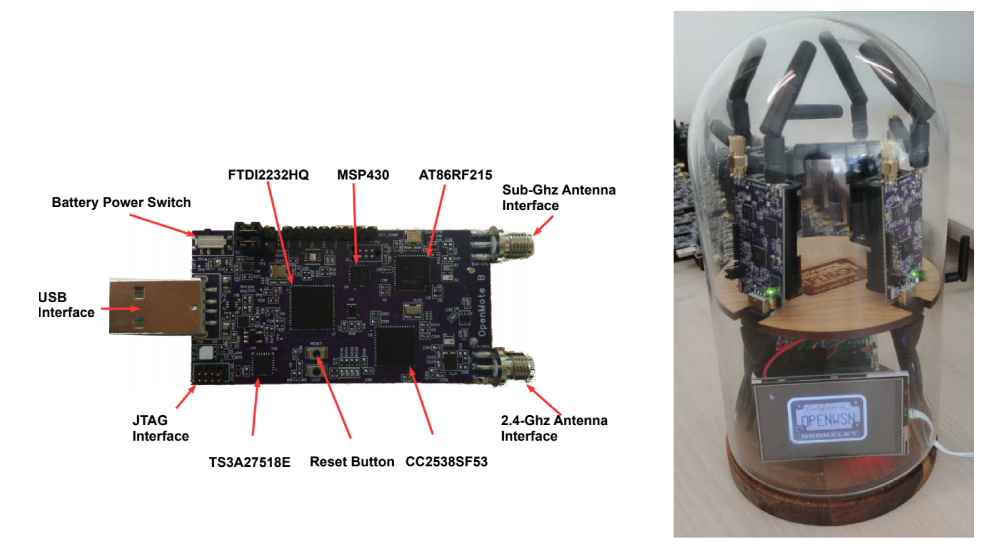
\includegraphics[width=0.90\columnwidth]{mote_ot}
	\caption{OpenMote B board (left) and The testbox containing four OpenMote B boards (right).}
    \label{fig:testbox}
\end{figure}

% 42-mote deployment

\lorem

\begin{figure}
	\centering
	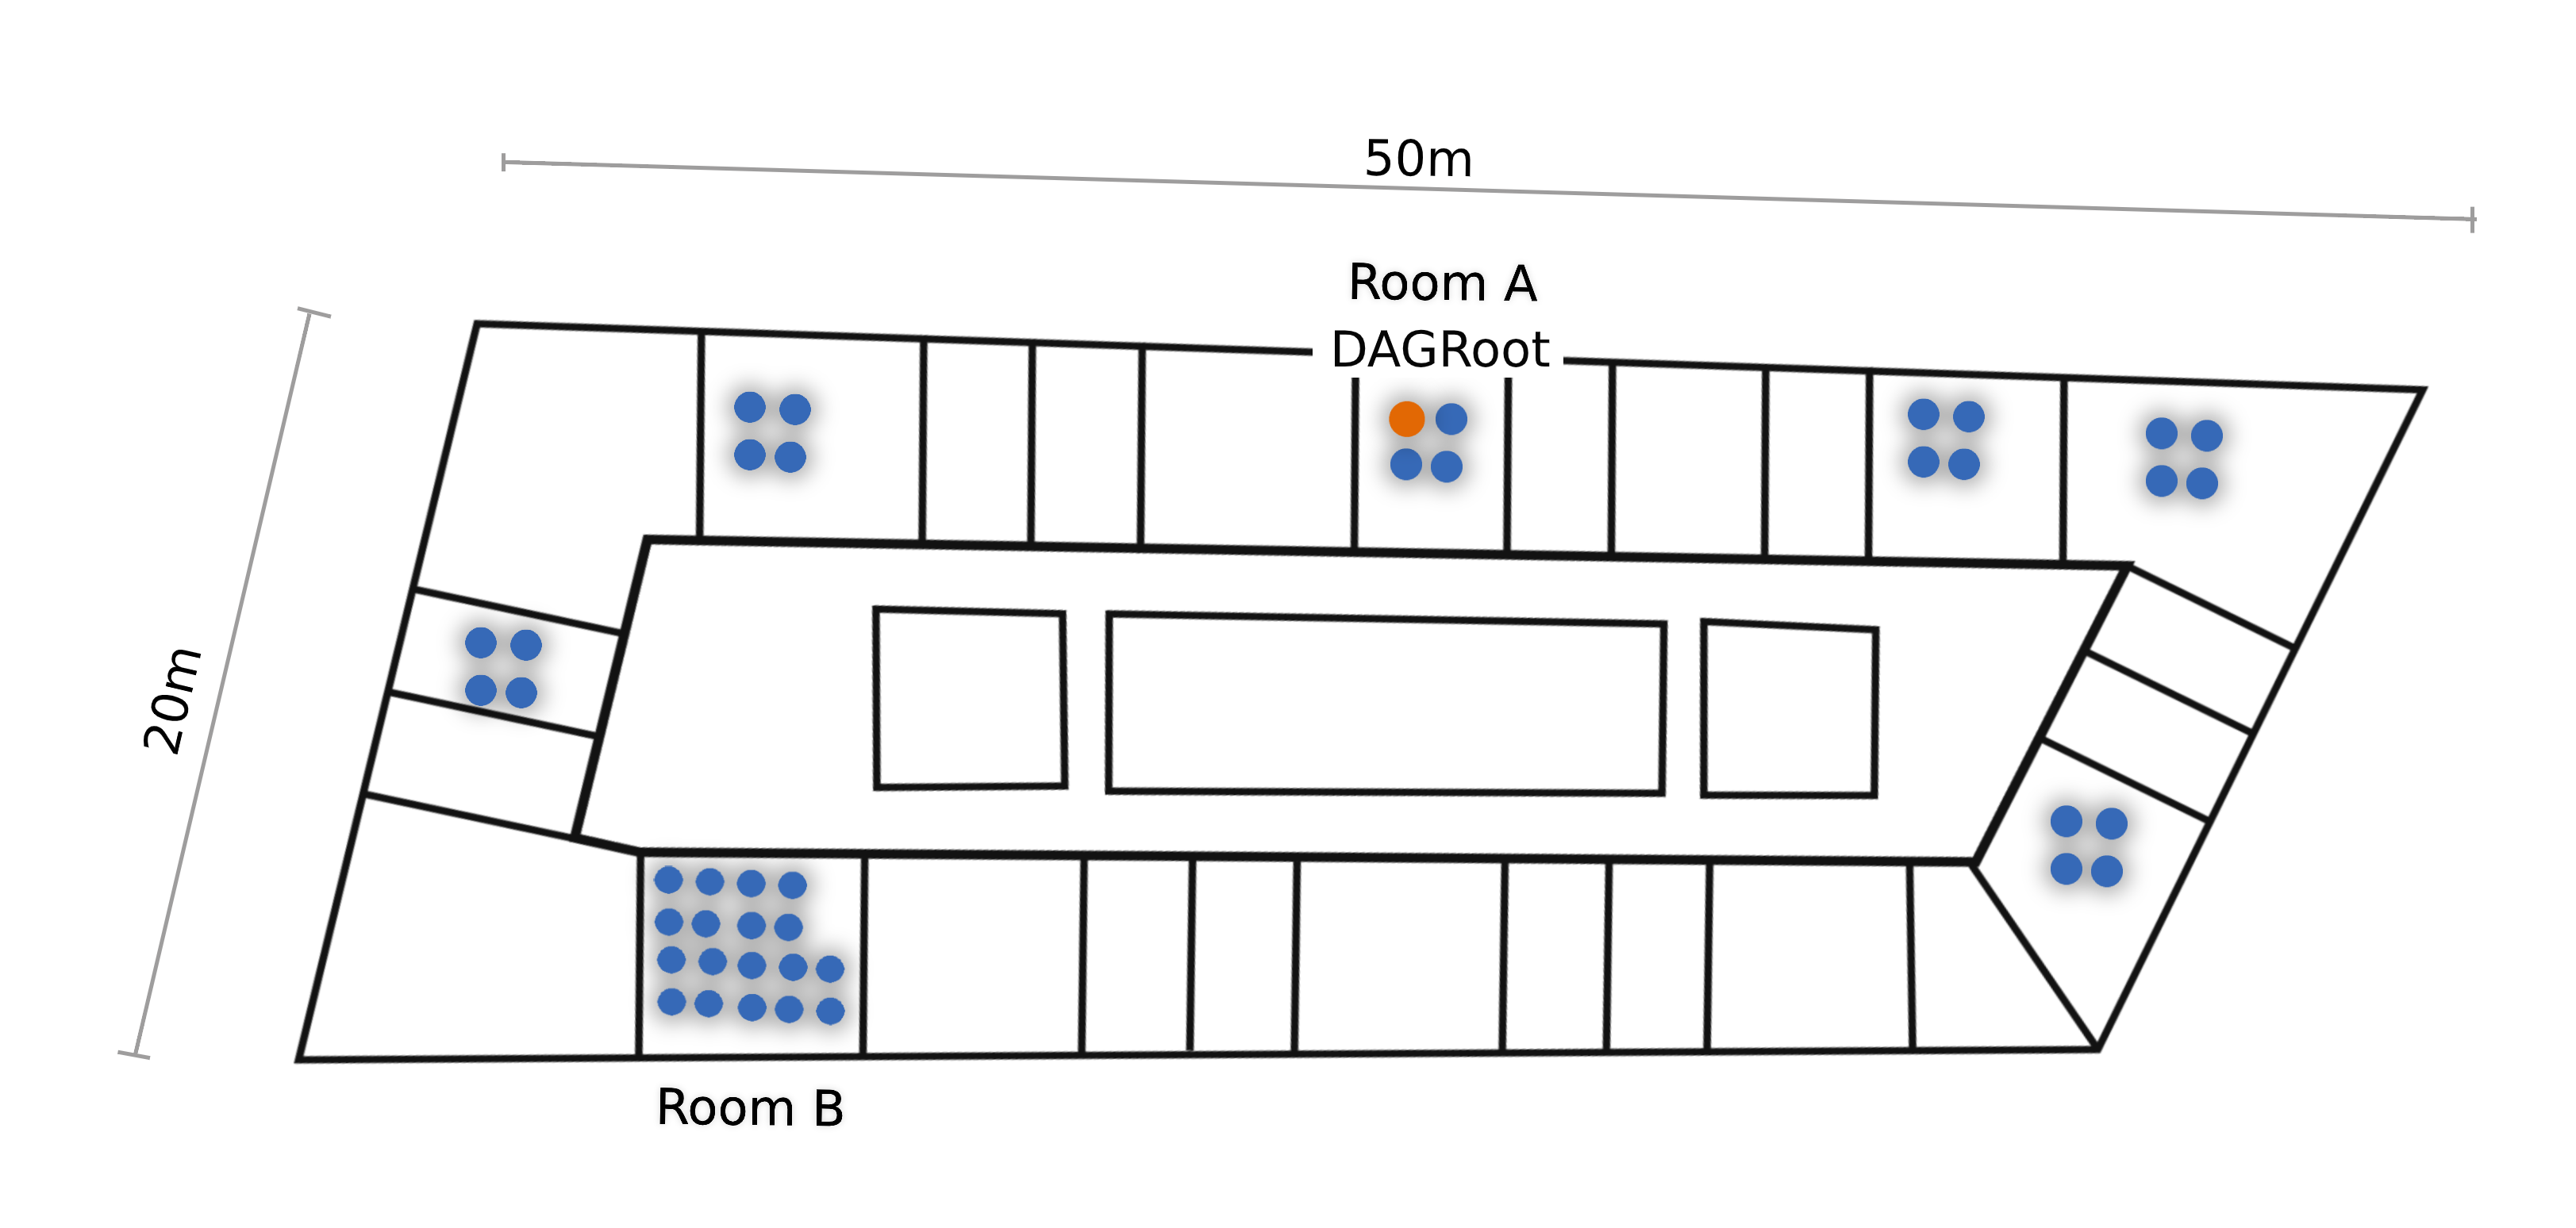
\includegraphics[width=0.90\columnwidth]{building_motes}
	\caption{Floorplan of the deployment.}
    \label{fig:floorplan}
\end{figure}

%==============================================================================
\section{A PHY-layer Agile Extension of OpenWSN}
\label{sec:openwsn}

% intro to 6TiSCH

\lorem

% intro to OpenWSN

\lorem

% goal: multiple PHY layer

\lorem \fsk \oqpsk \ofdm``FSK\_subGHz''

% OpenWSN Extension

\lorem

% result: footprint

\lorem

%==============================================================================
\section{Methodology}
\label{sec:methodology}

% repeating 3 times

\lorem

% duration of one experiment

\lorem

% gathering data, publishing raw results, etc.

\lorem

% KPIs

\lorem

% running the experiments

\lorem

%==============================================================================
\section{Experimental Results}
\label{sec:results}

\lorem

%------------------------------------------------------------------------------
\subsection{Network Formation}
\label{sec:network_formation}

% why is it important, define

\lorem

% worst case from a contention point of view

\lorem

% results

\lorem Fig.~\ref{fig:time_firstpacket_cdf}

\begin{figure}
	\centering
	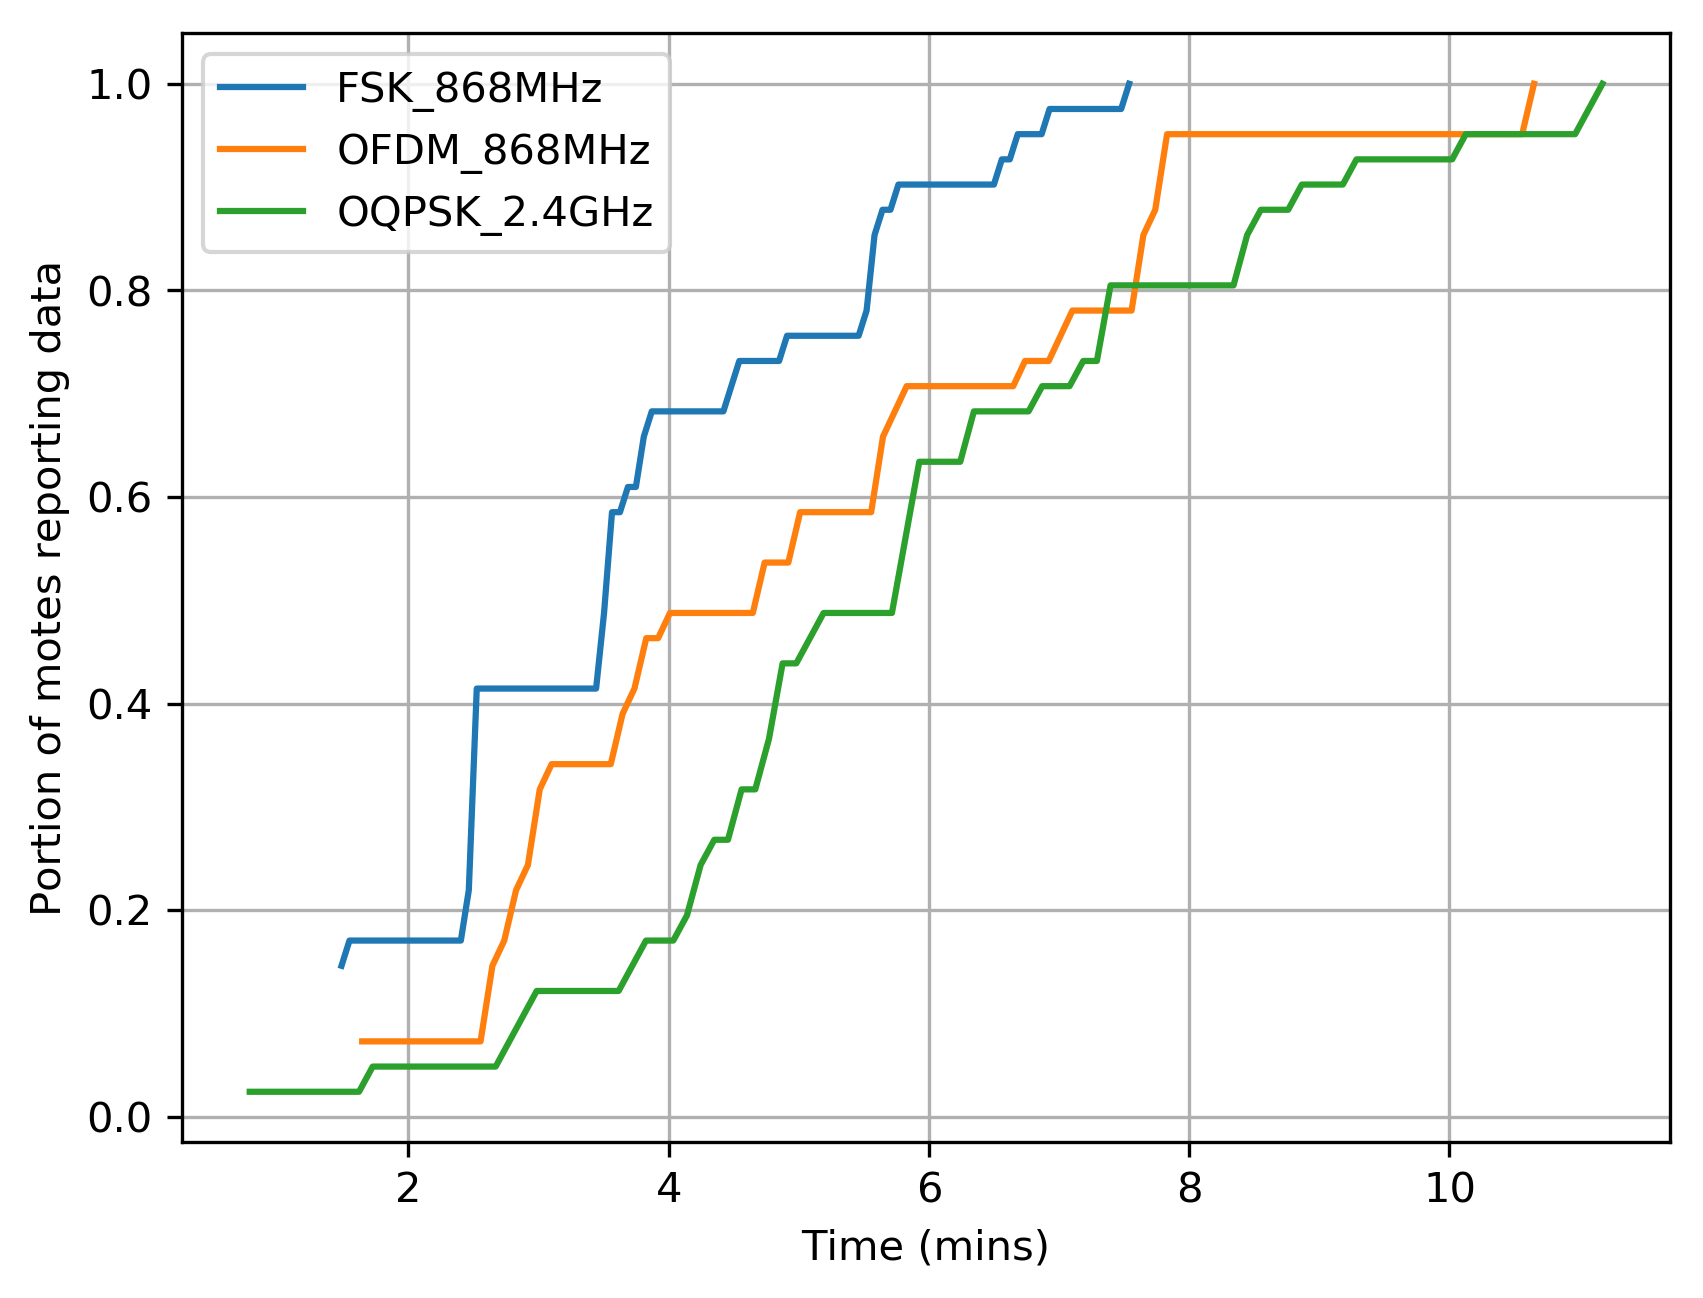
\includegraphics[width=0.90\columnwidth]{time_firstpacket_cdf}
	\caption{Time to First Packet CDF.}
    \label{fig:time_firstpacket_cdf}
\end{figure}

% settling time, steady-state   

\begin{figure}
	\centering
	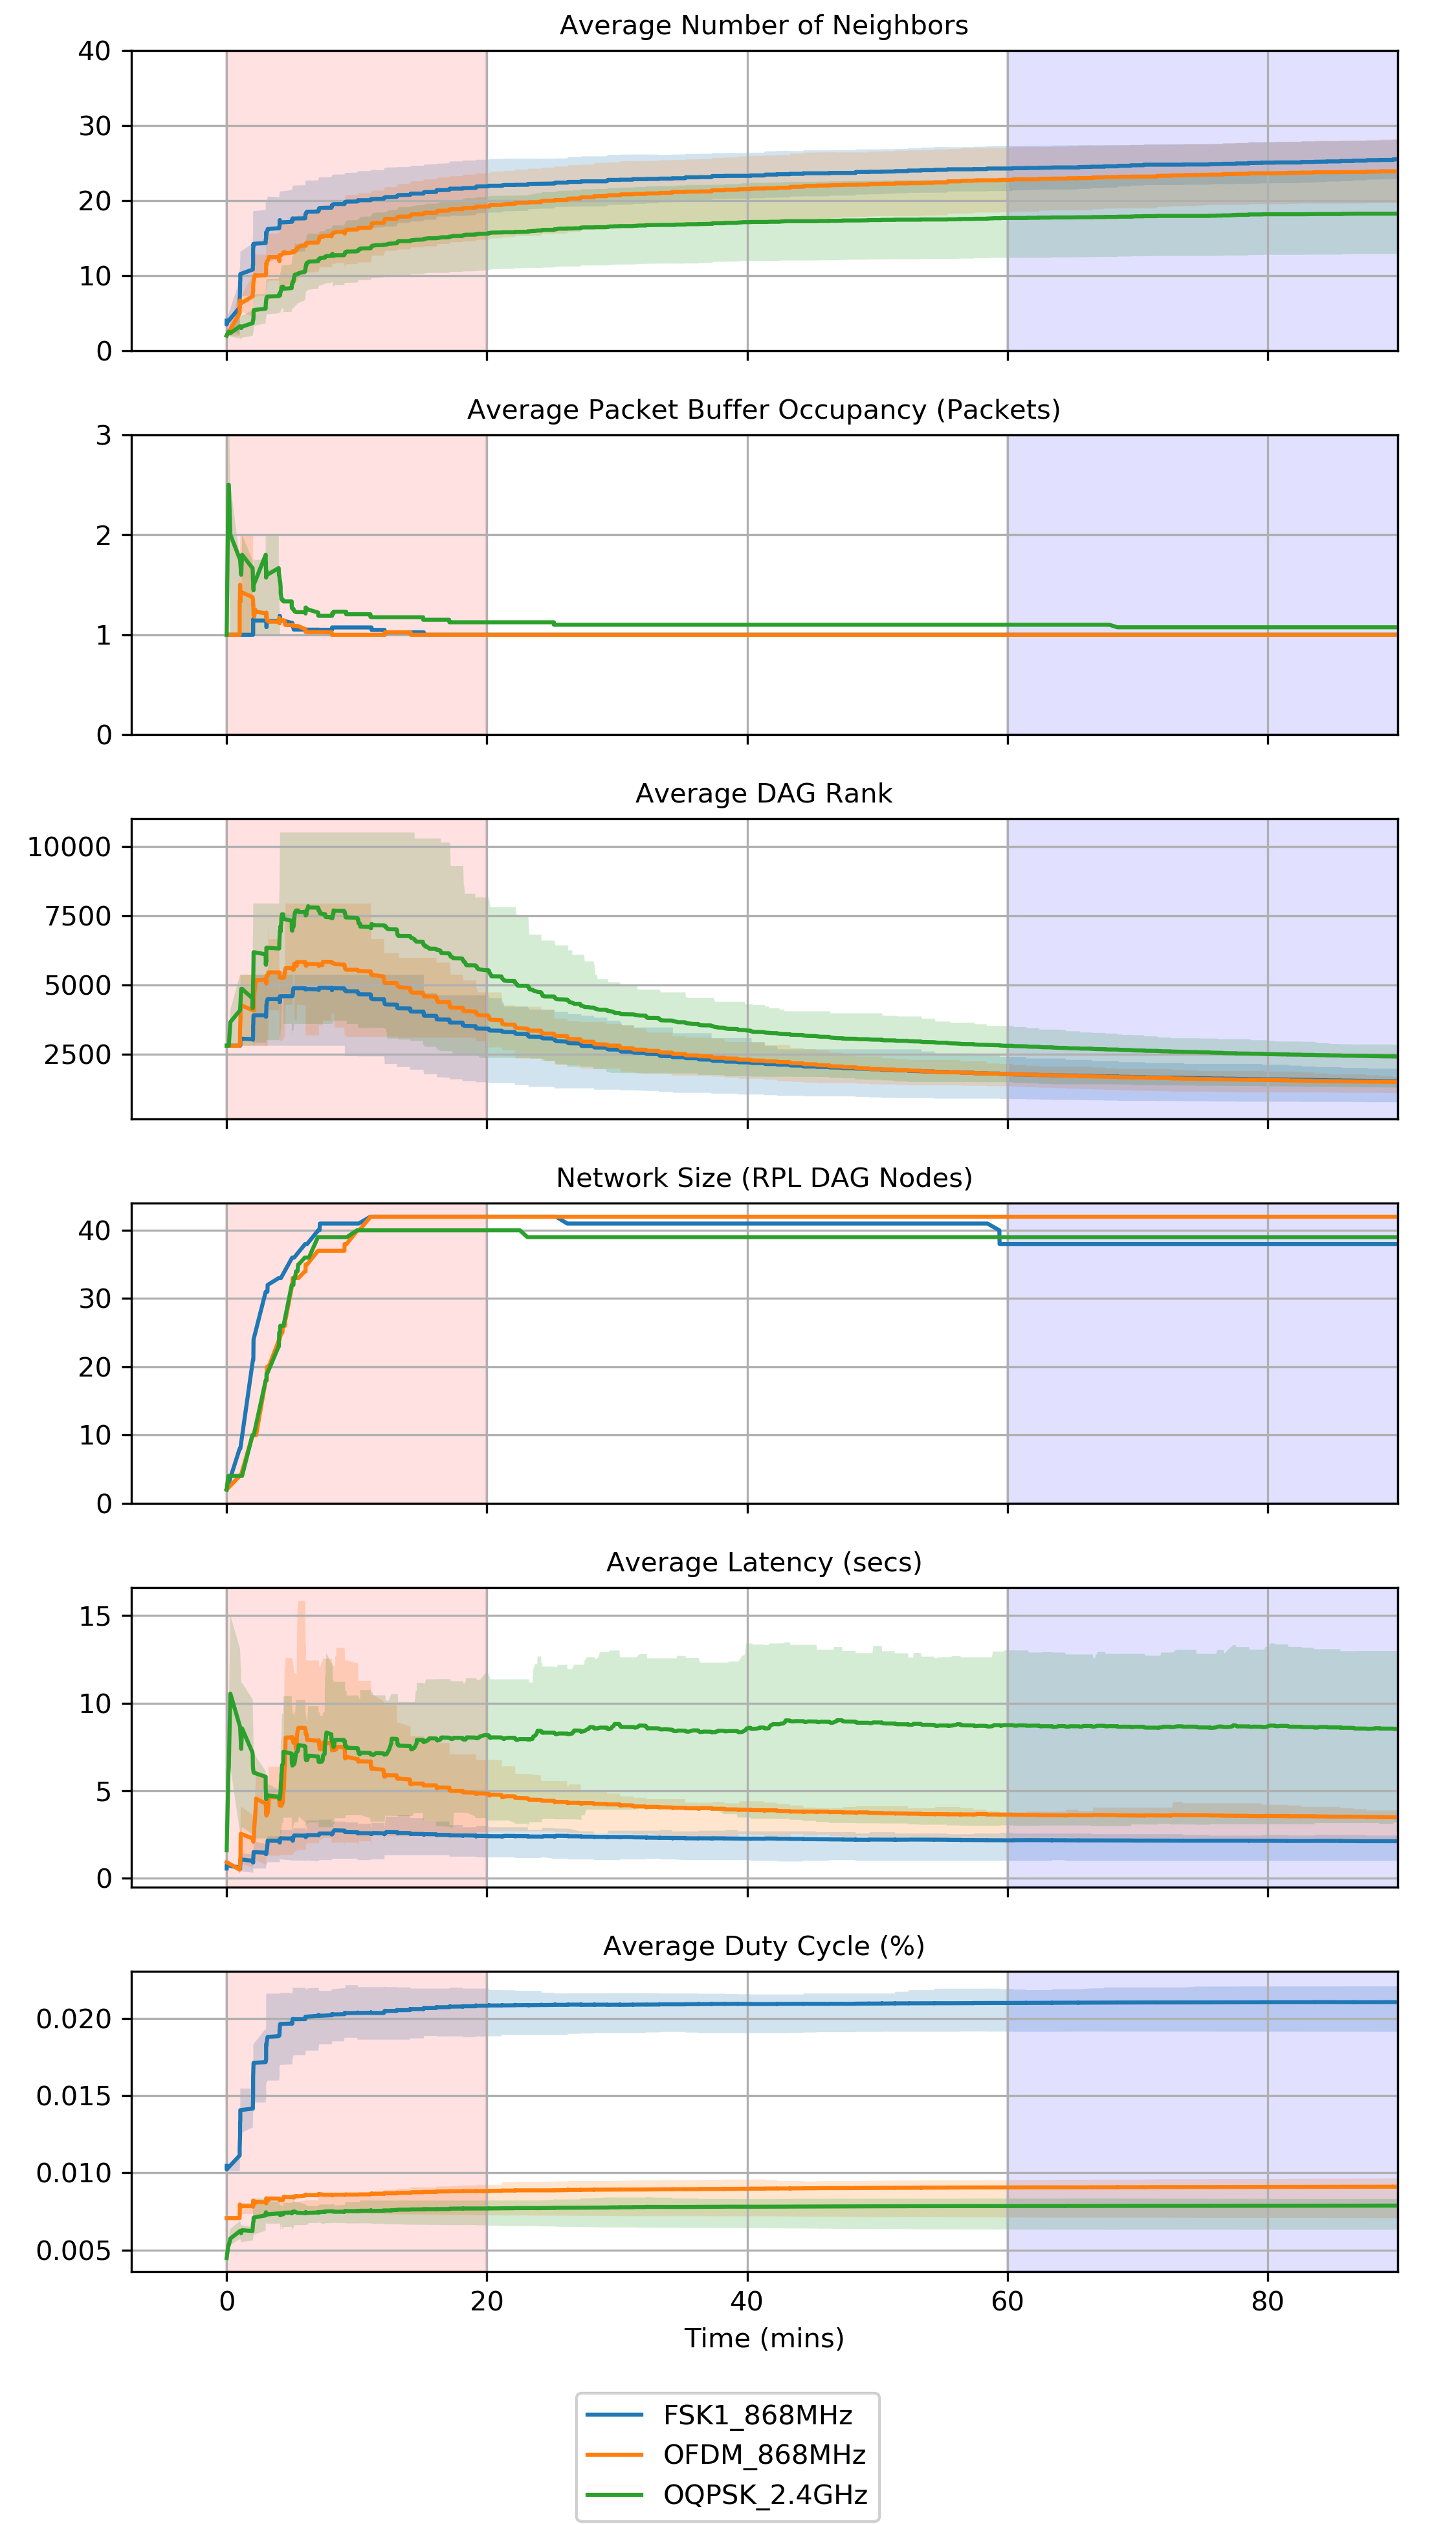
\includegraphics[width=0.90\columnwidth]{aggregate_plot_reliability}
	\caption{6TiSCH reliability performance under each radio setting in the three stages of network formation: 1) discovery and formation phase (red highlight),and 2) steady-state phase (blue highlight). Shaded curves represent the majority of the distribution (interquartile range)}
    \label{fig:aggregate_plot_reliability}
\end{figure}


%------------------------------------------------------------------------------
\subsection{End-to-End Reliability}
\label{sec:reliability}
% why is it important, and how is it measured? 
% Packet loss on shared cells. 
% Long range lead to more neighbors which leads to discovery of better neighbors closer to the root. 

% The negative side is that requires more active and strict rule for accepting neighbors, otherwise it would lead to a neighbor table buffer overflow, specially in dense networks

% Short range can cause more packet loss due to lower link budget if propagation is challenging. 


\begin{table}
 \caption {Steady-state end-to-end PDR values} \label{tab:pdr_table} 
 \begin{center}
 \begin{tabular}{||c c c c||} 
 \hline
 Radio Setting & Average & Median & Stdev \\ [0.5ex] 
 \hline\hline
 \fsk & 100\% & 100\% & 0 \\ 
 \hline
 \ofdm & 99,9521\% & 100\% & 0.302 \\
 \hline
 \oqpsk & 100\% & 100\% & 0 \\
 \hline

\end{tabular}
\end{center}
\end{table}


\begin{figure}
	\centering
	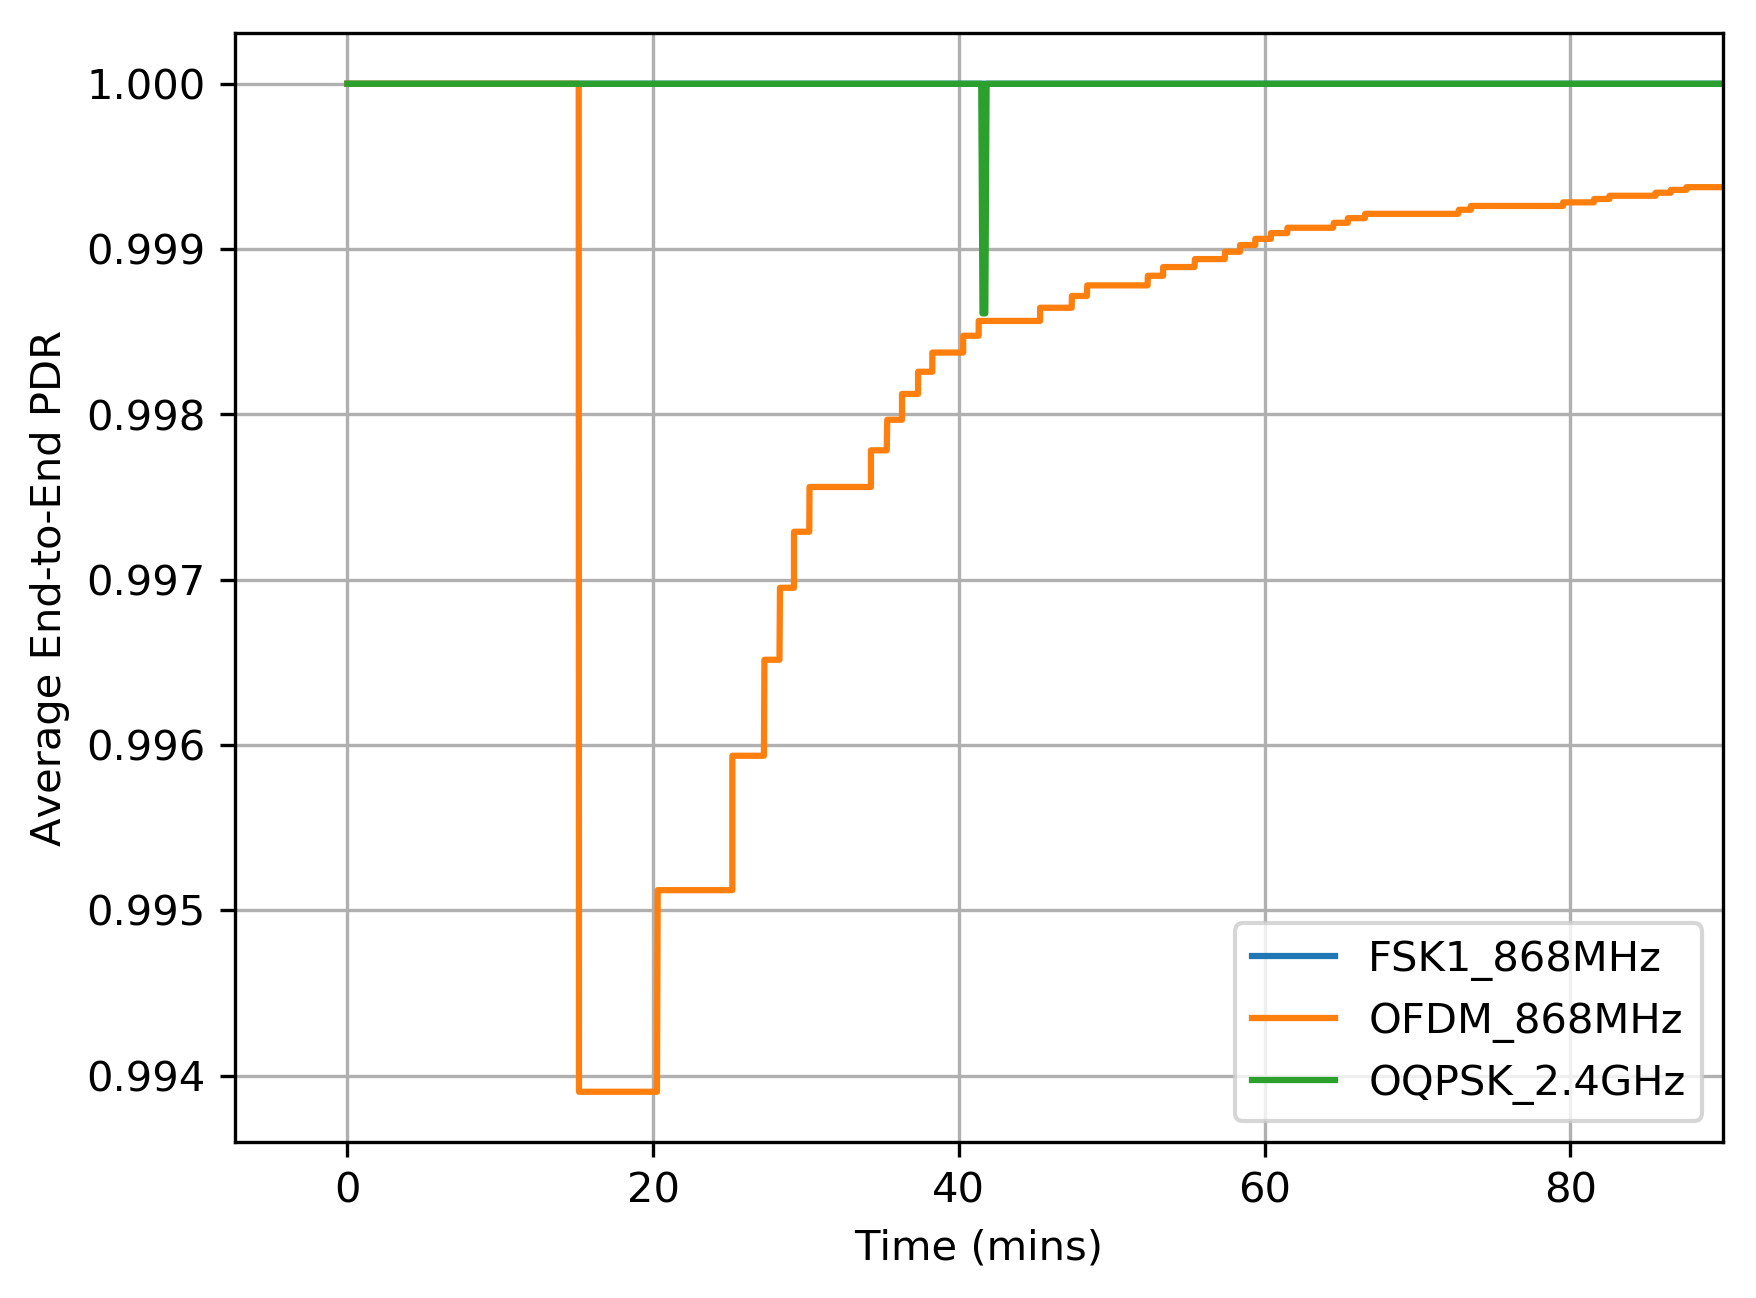
\includegraphics[width=0.9\columnwidth]{avg_pdr_plot.png}
	\caption{Average end-to-end PDR. }
    \label{fig:avg_pdr_plot}
\end{figure} 

%------------------------------------------------------------------------------
\subsection{End-to-End Latency}
\label{sec:latency}

% why is this important? information recency, alarms, logging of critical events for the reactive or preemptive measures.
% higher link budget lead to discovery of more neighbors which leads less hops and less end to end latency.

% shorter range not only suffer from more hops but also more re-transmissions.

\begin{figure}
	\centering
	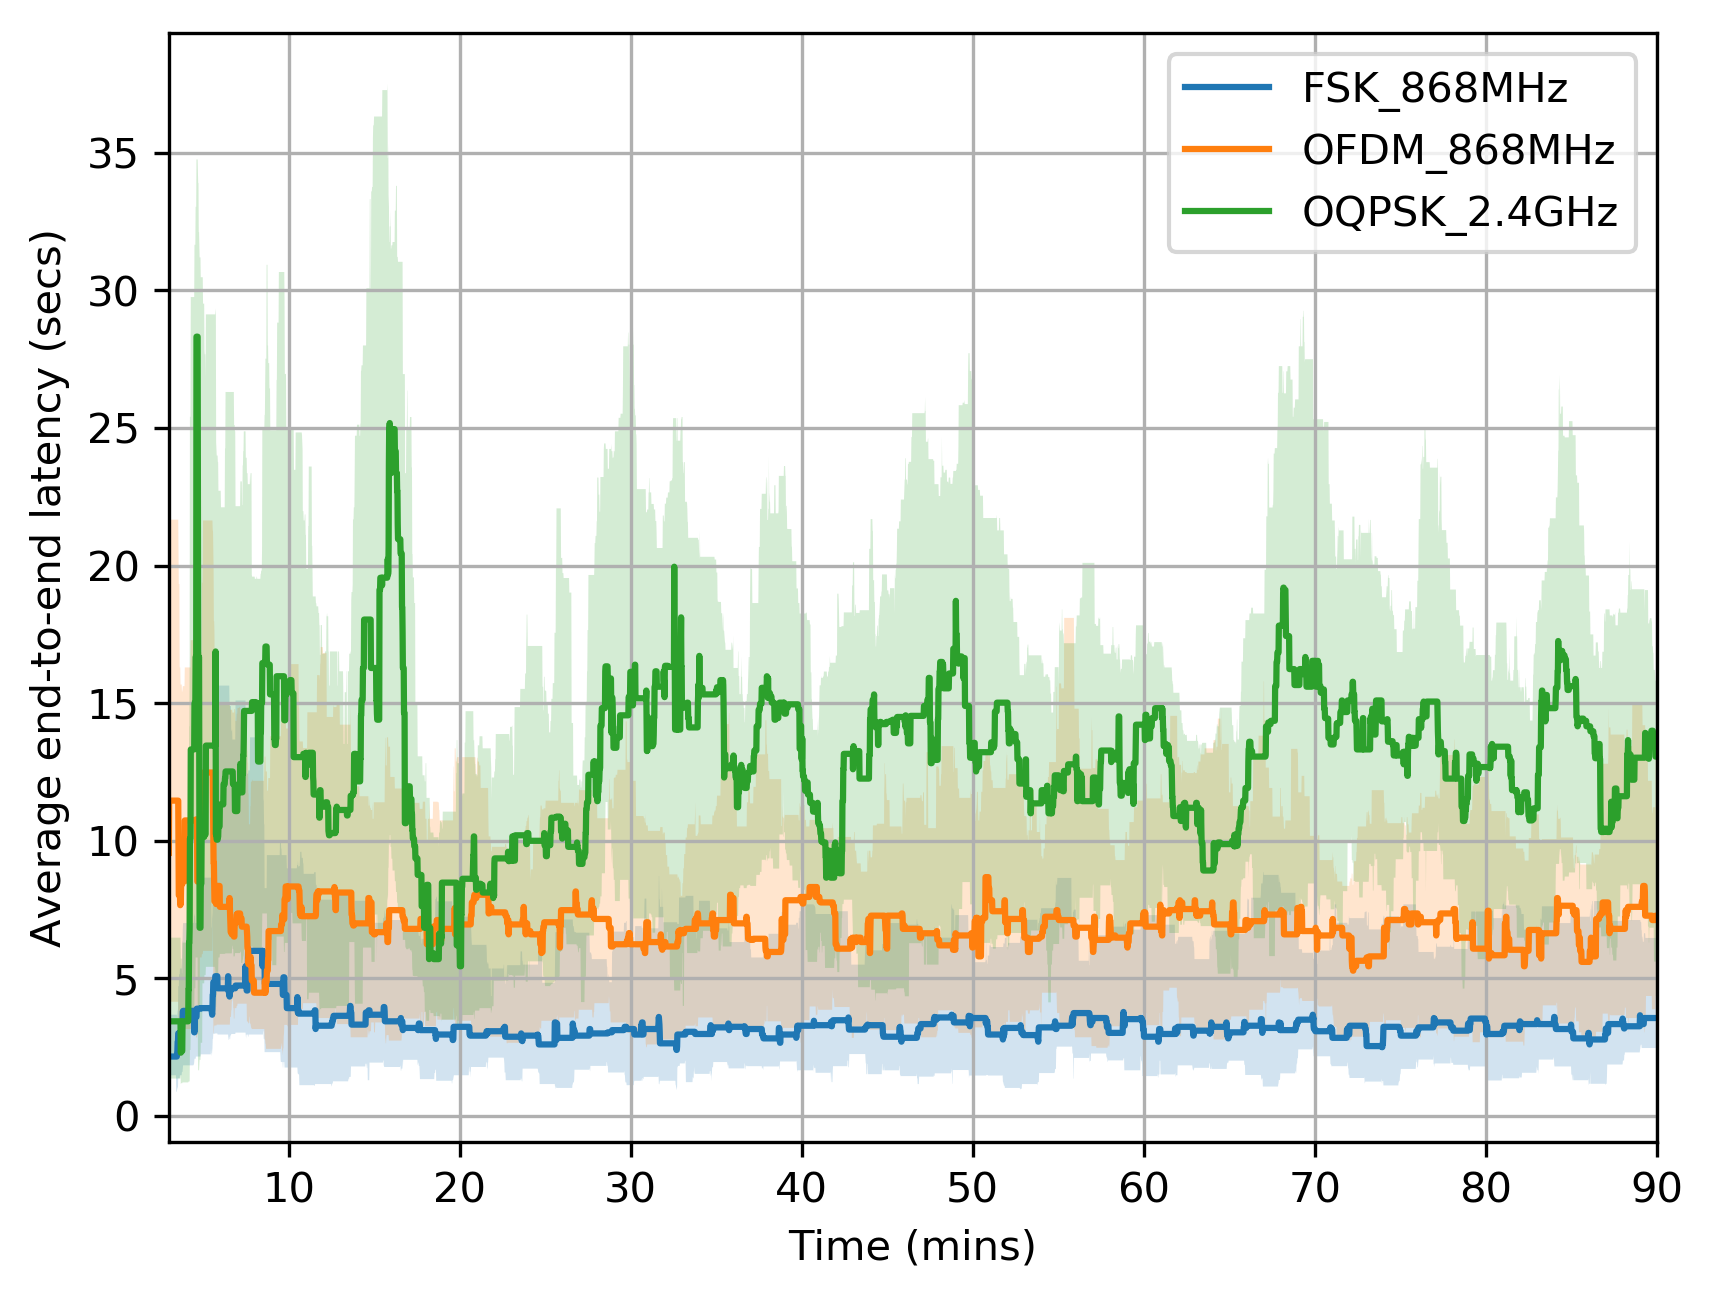
\includegraphics[width=0.90\columnwidth]{avg_latency_plot}
	\caption{Average end-to-end latency. Shaded curves represent the majority of the distribution - i.e. interquartile range (extracted from Fig. \ref{fig:aggregate_plot_reliability})}
    \label{fig:avg_latency_plot}
\end{figure}

%------------------------------------------------------------------------------
\subsection{Queue Occupancy}
\label{sec:queue}


% why is this important? memory limitations, packet loss simply due to unavailable buffer space. 

% Interestingly enough, it seems that there is an inverse correlation between bit-rate and average packet buffer occupancy as seen in Fig.~\ref{fig:avg_bufferSize_plot}. 

% In this setting, the packet queue buffer is of size 20 entries. 



\begin{figure}
	\centering
	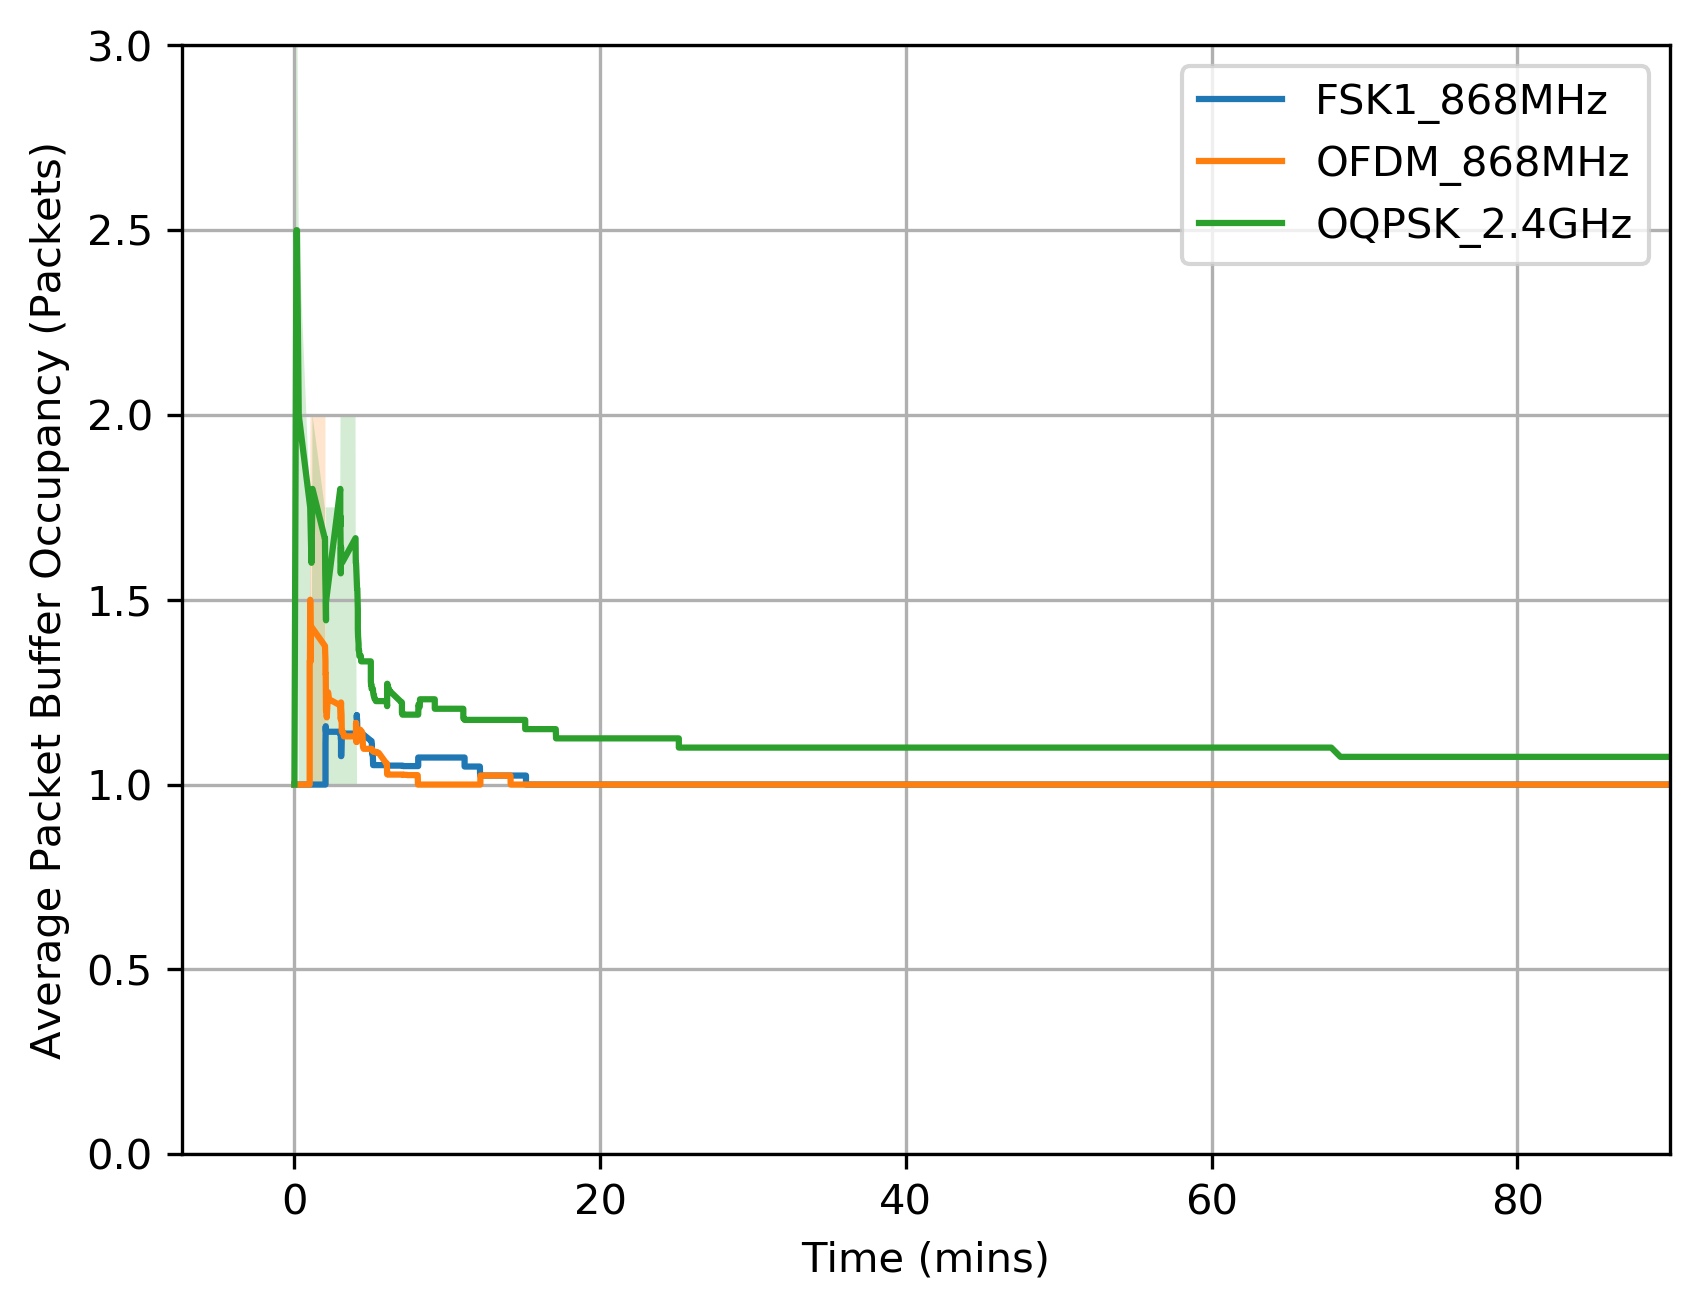
\includegraphics[width=0.90\columnwidth]{avg_bufferSize_plot}
	\caption{Average queue occupancy (extracted from Fig. \ref{fig:aggregate_plot_reliability})}
    \label{fig:avg_bufferSize_plot}
\end{figure}

%------------------------------------------------------------------------------
\subsection{Battery Lifetime}
\label{sec:battery_lifetime}


% why is this important? essential opex. OpEx presents a huge constraint and could lead to impractical deployment if batteries have to change too often (thesis reference)
\begin{figure}
	\centering
	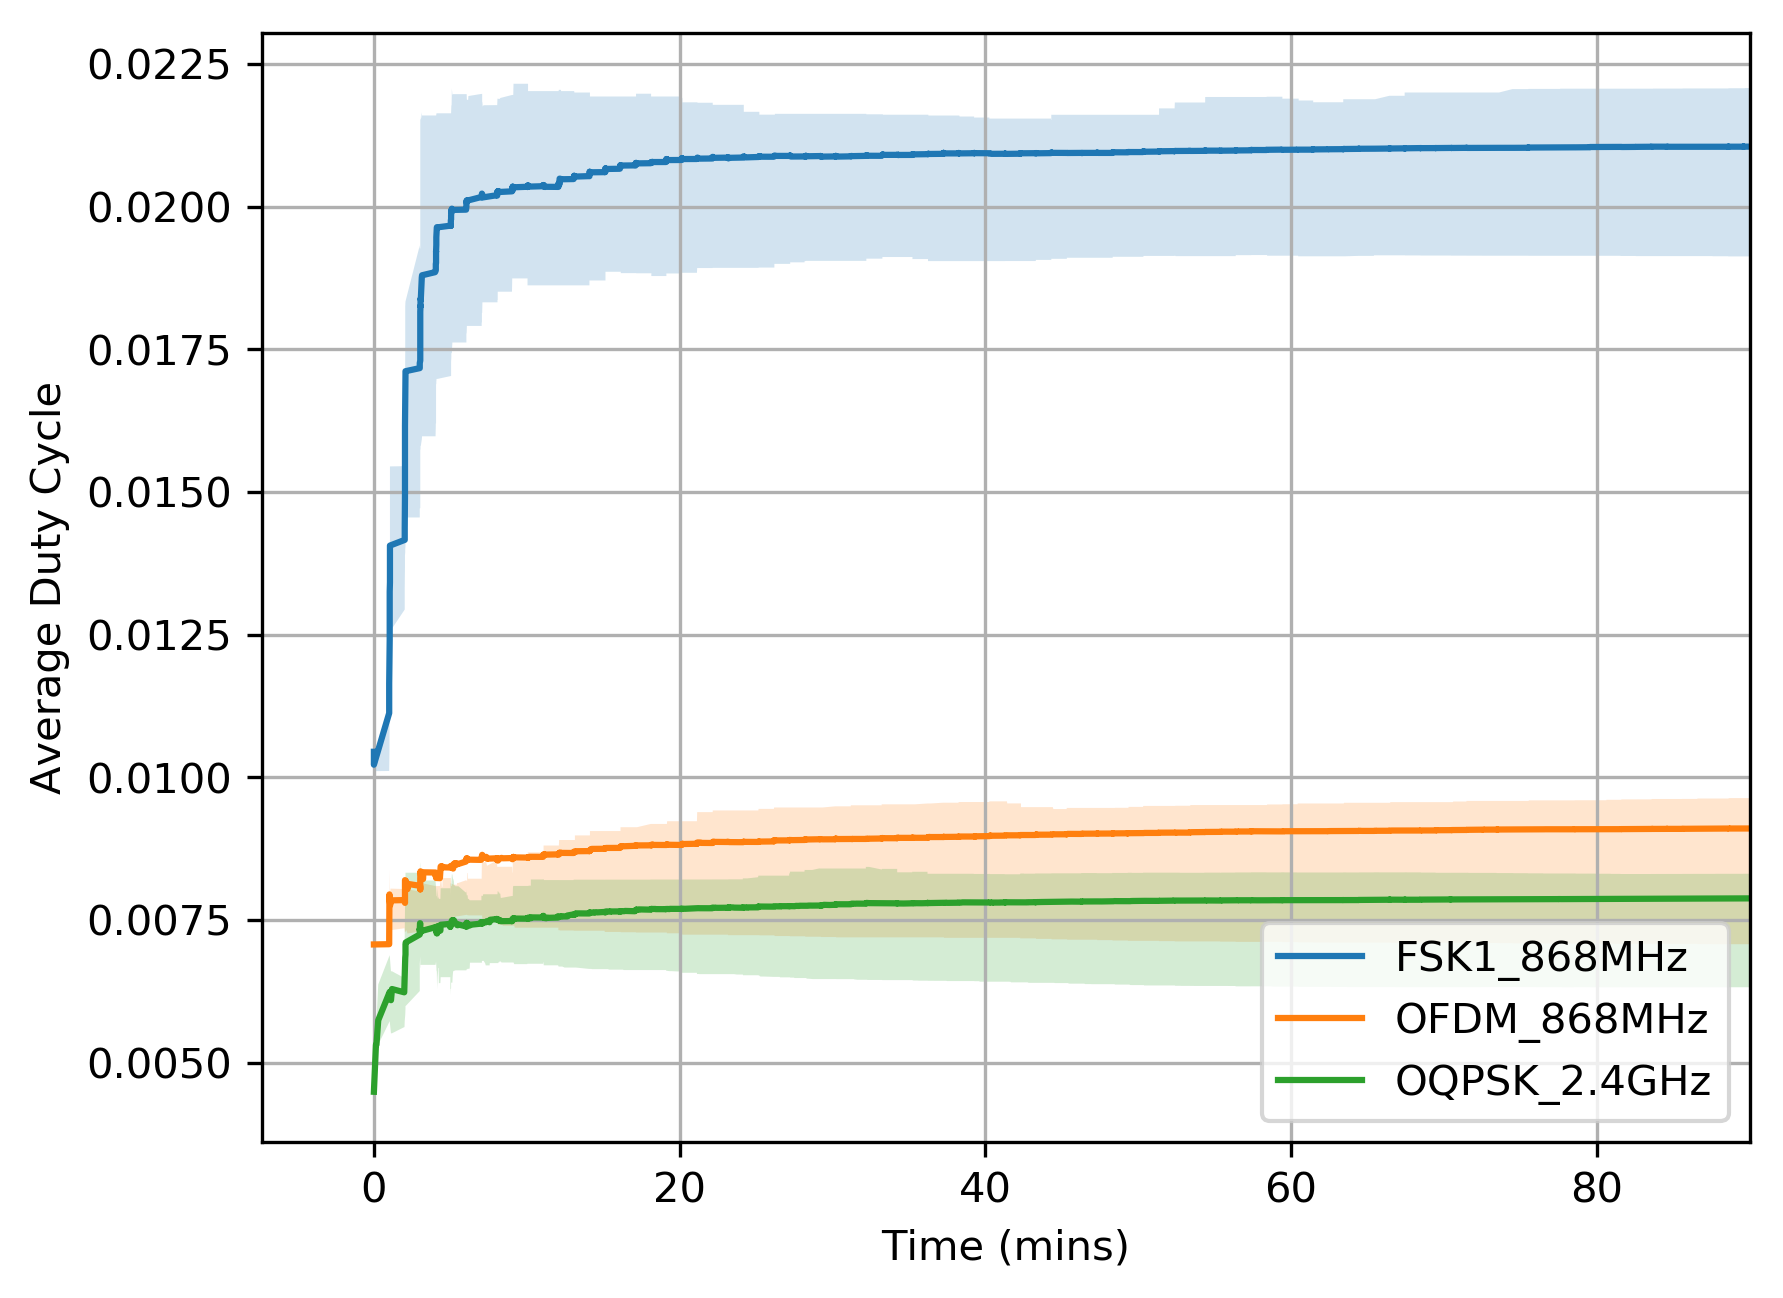
\includegraphics[width=0.90\columnwidth]{avg_avg_dutyCycle_plot}
	\caption{Average duty cycle.Shaded curves represent the majority of the distribution - i.e. interquartile range. (extracted from Fig. \ref{fig:aggregate_plot_reliability})}
    \label{fig:avg_avg_dutyCycle_plot}
\end{figure}

%------------------------------------------------------------------------------
\subsection{Cumulative Comparison of the Results}
\label{sec:cimulative}



\begin{figure}
	\centering
	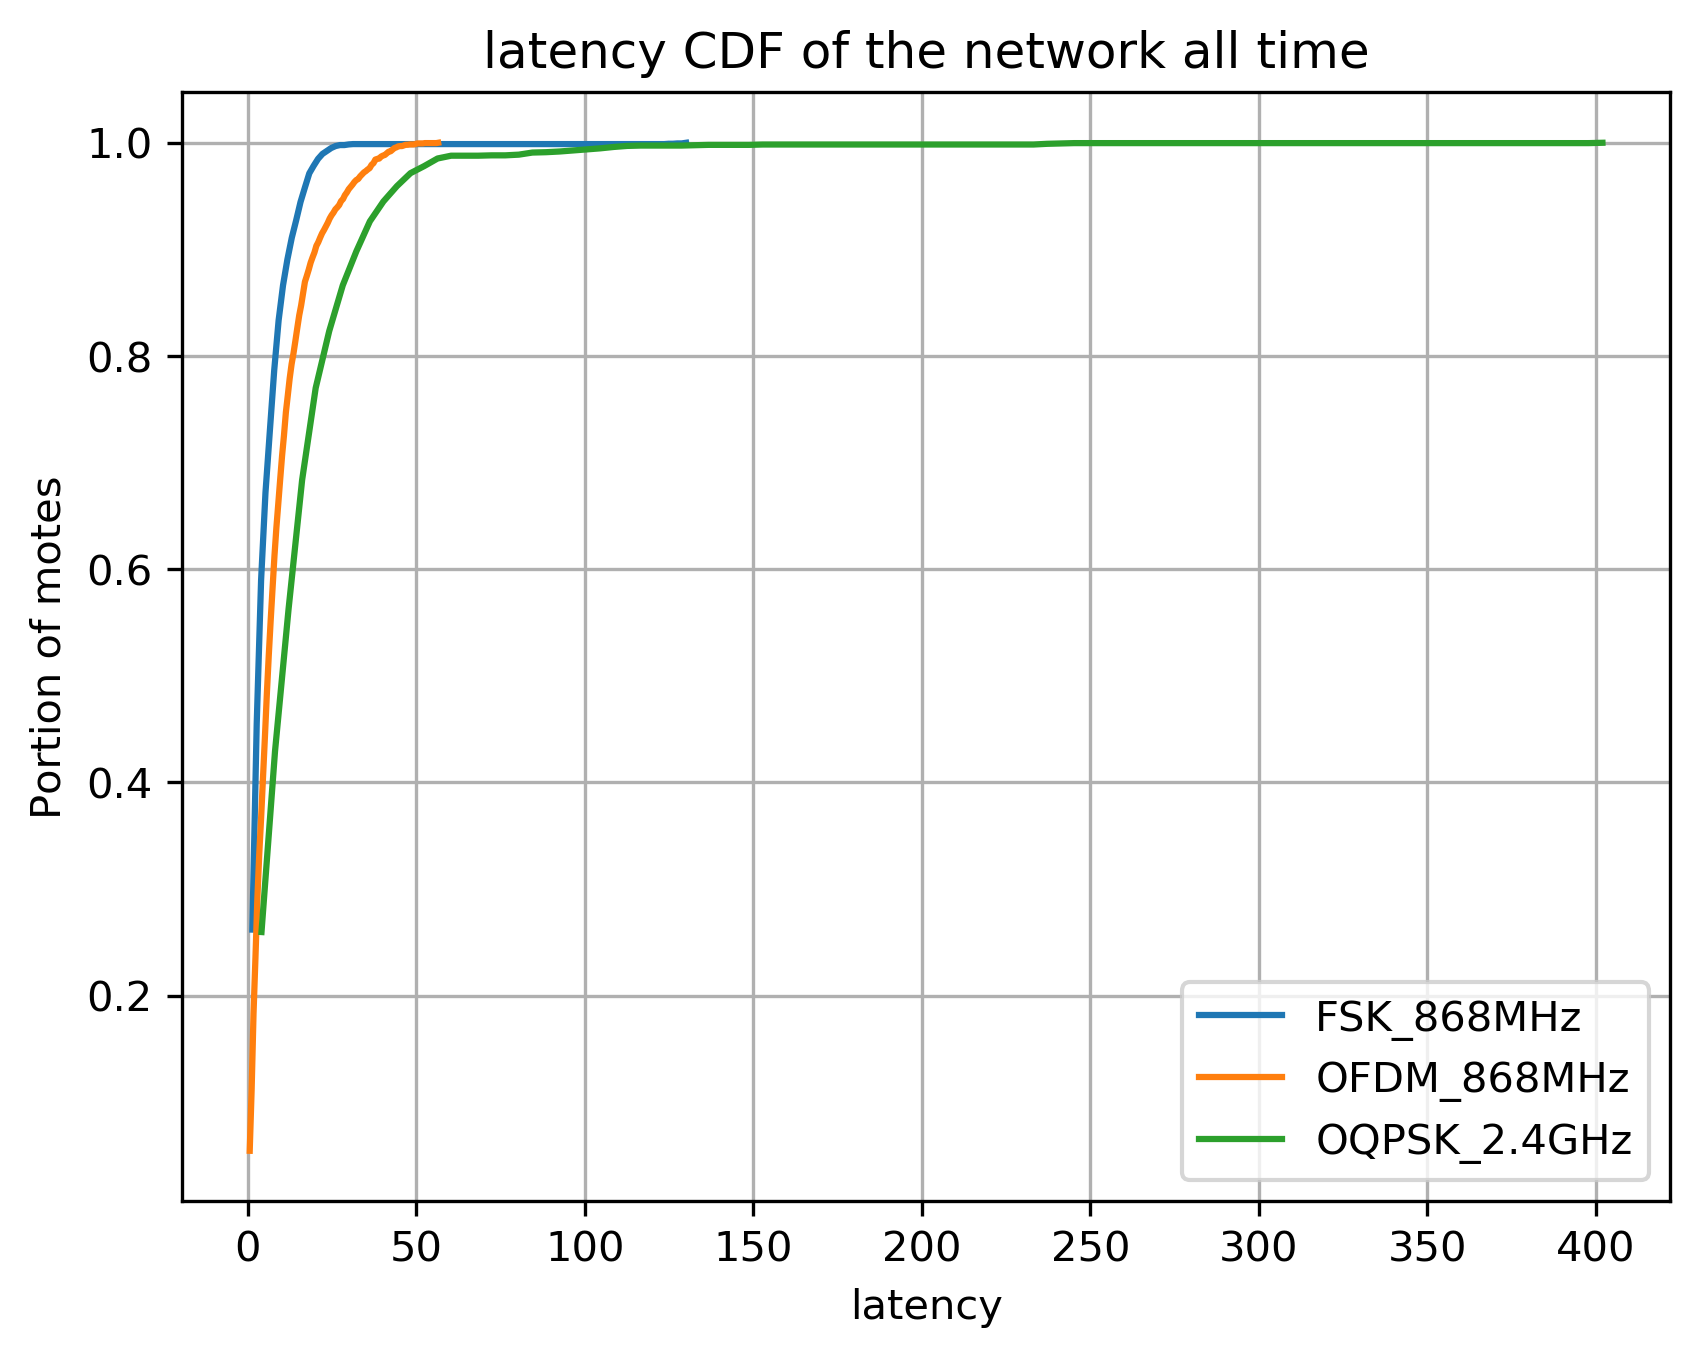
\includegraphics[width=0.90\columnwidth]{latency_cdf_plot_full}
	\caption{CDF of latency in the network} 
    \label{fig:latency_cdf_plot_full}
\end{figure}

\begin{figure}
	\centering
	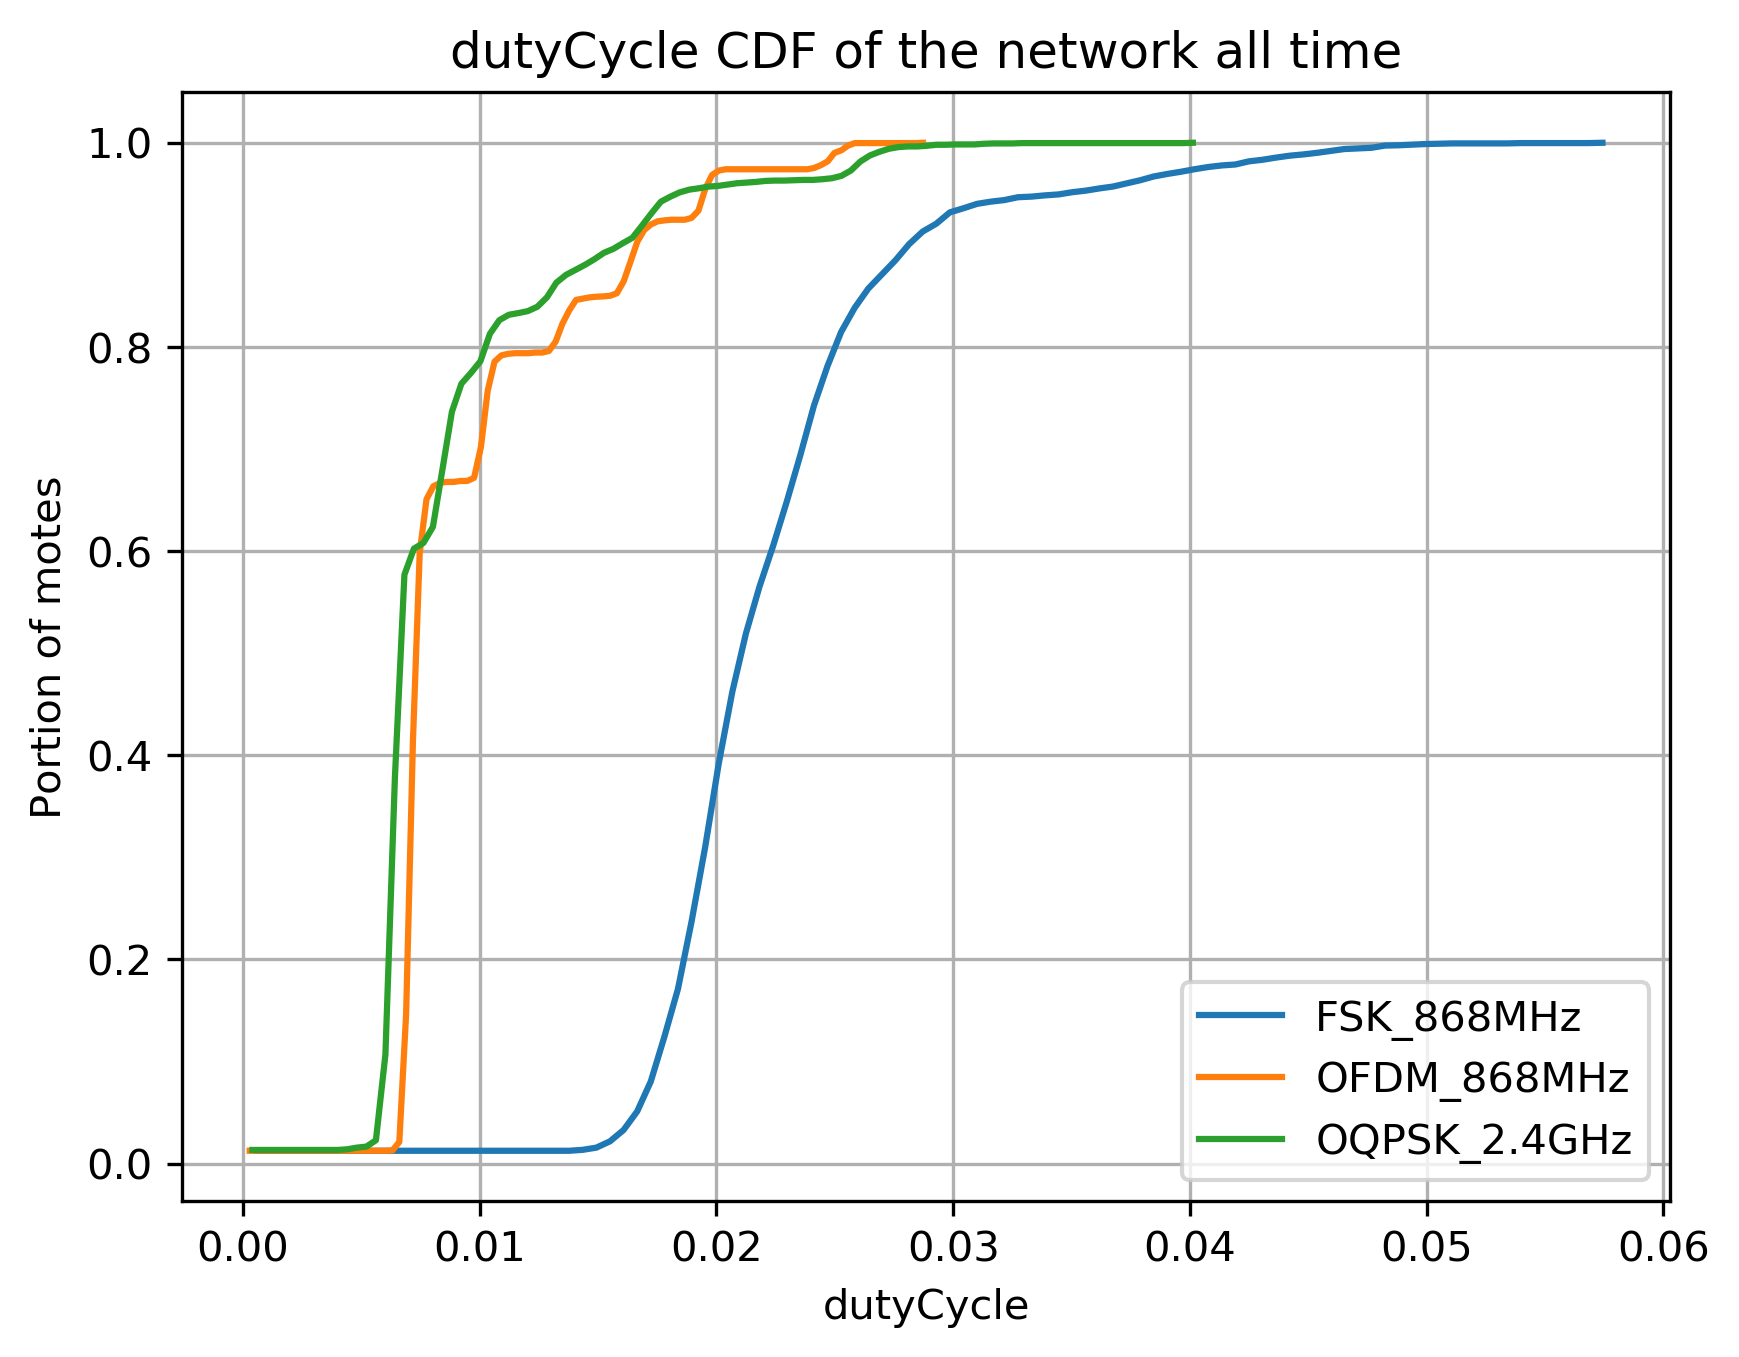
\includegraphics[width=0.90\columnwidth]{dutyCycle_cdf_plot_full}
	\caption{CDF of radio duty cycle in the network} 
    \label{fig:dutyCycle_cdf_plot_full}
\end{figure}

\begin{figure}
	\centering
	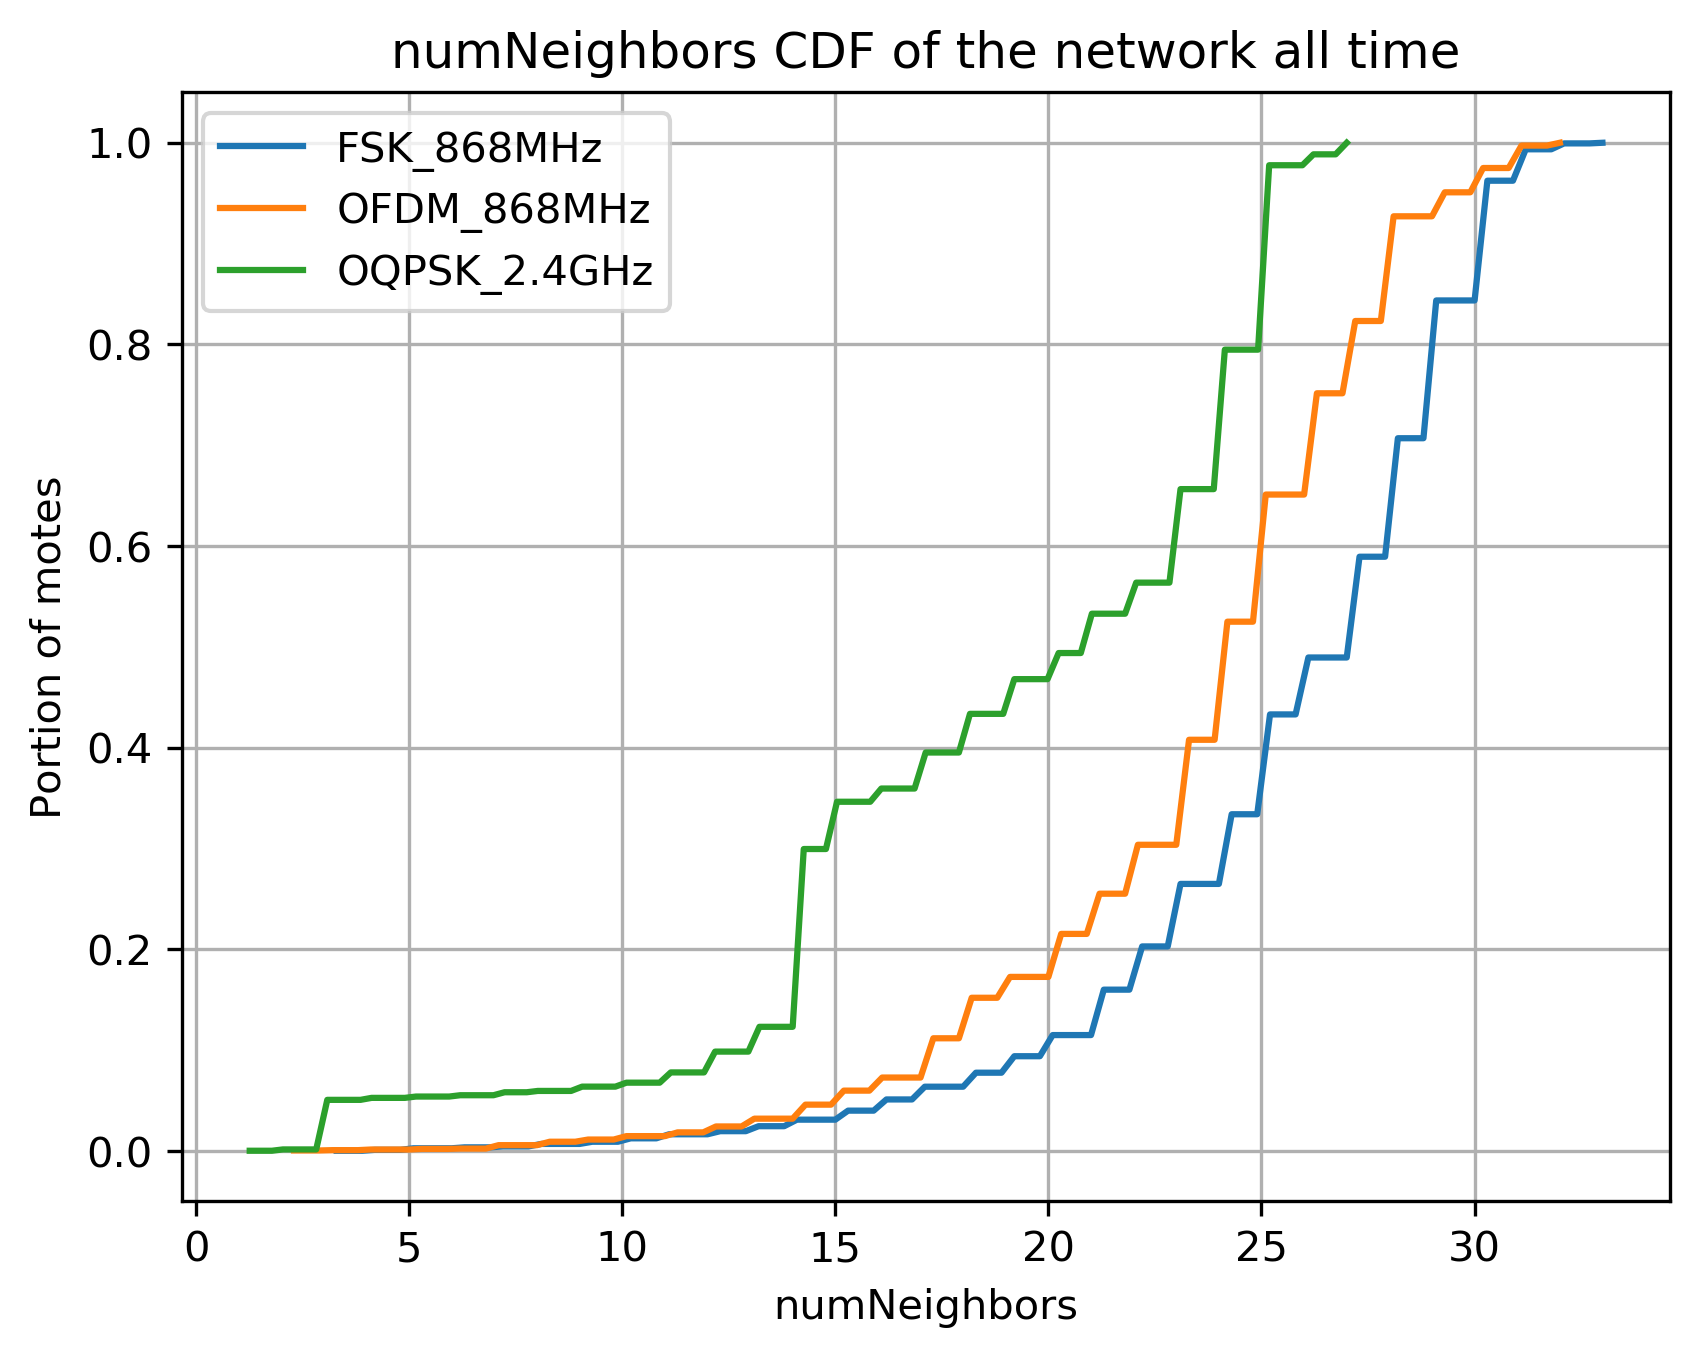
\includegraphics[width=0.90\columnwidth]{numNeighbors_cdf_plot_full}
	\caption{CDF of number of neighbors in the network} 
    \label{fig:numNeighbors_cdf_plot_full}
\end{figure}

\begin{figure}
	\centering
	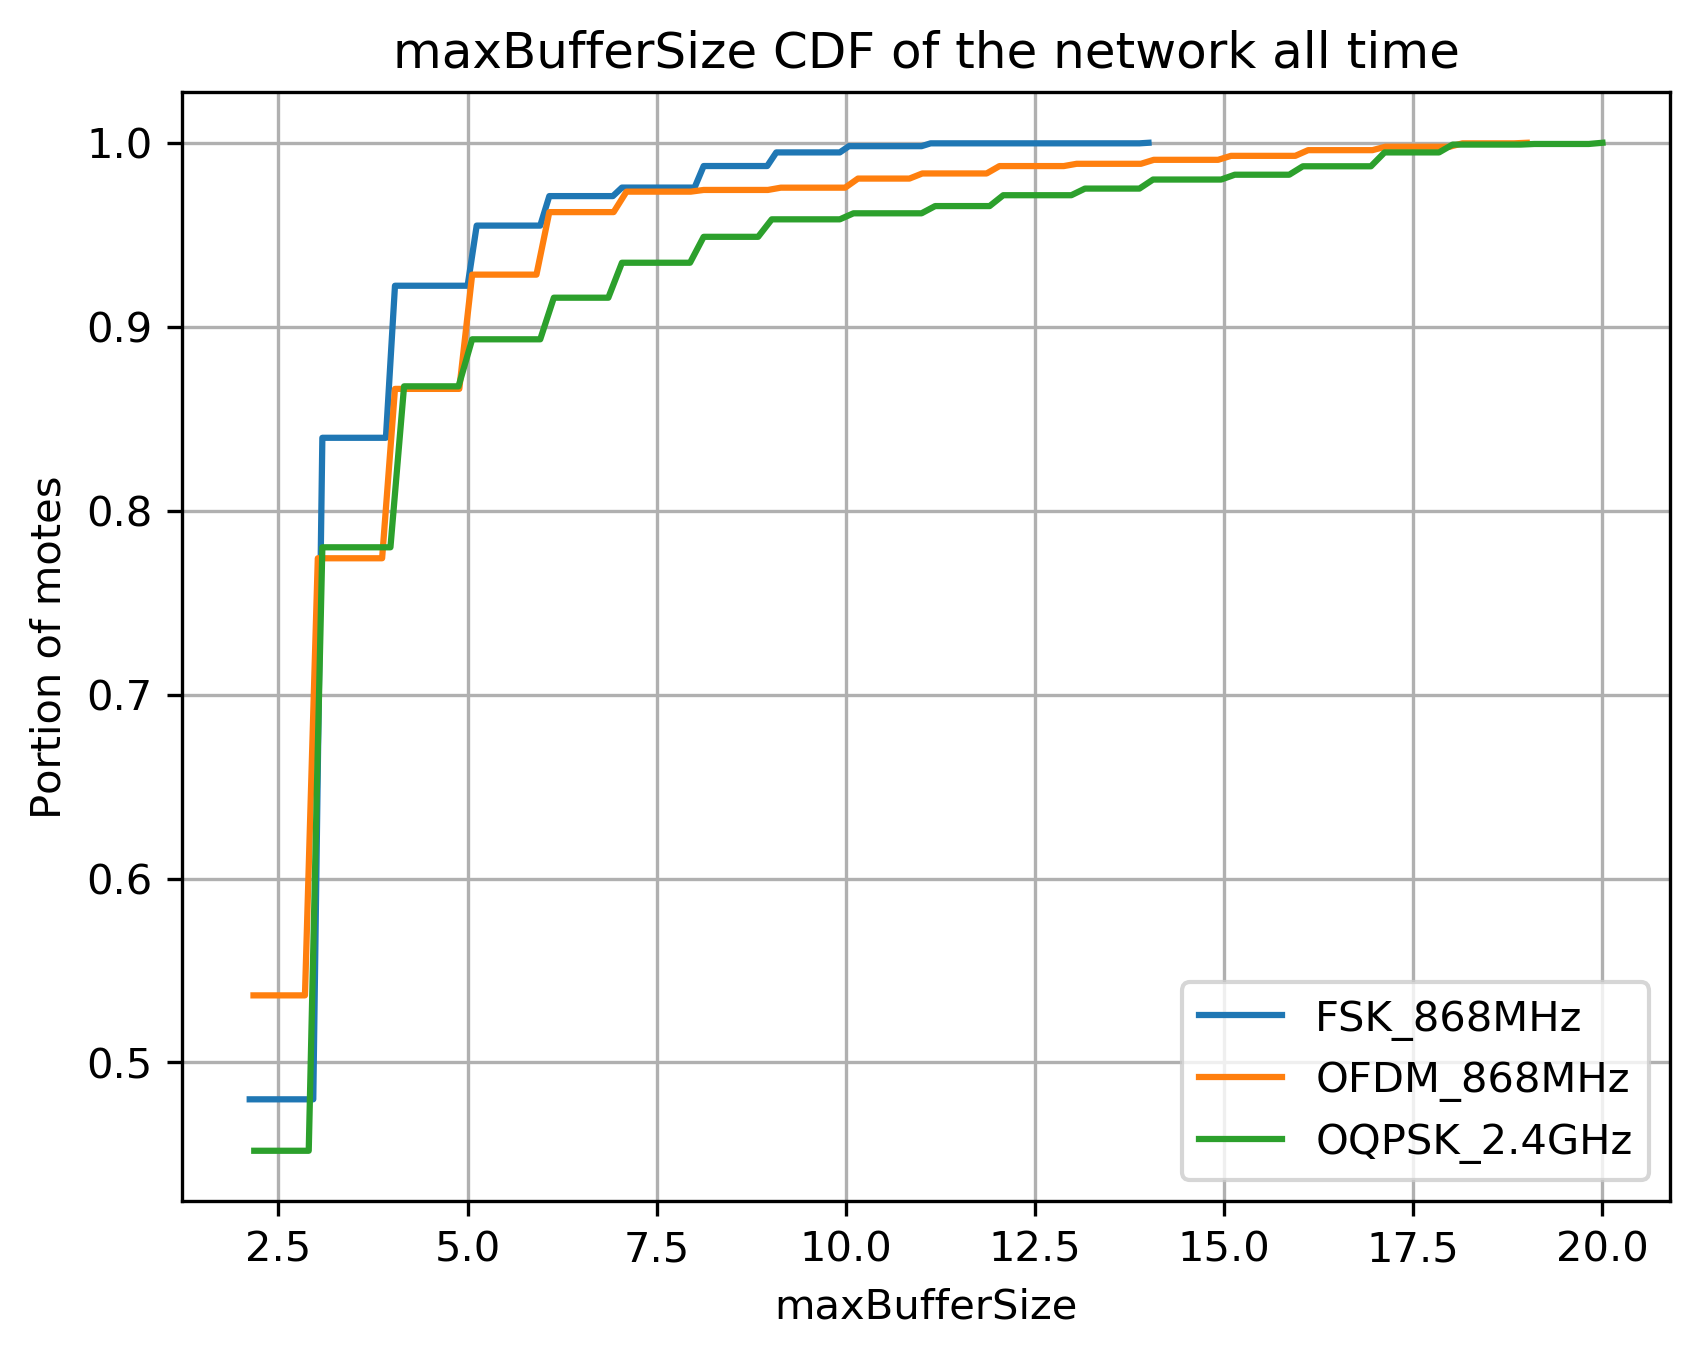
\includegraphics[width=0.90\columnwidth]{maxBufferSize_cdf_plot_full}
	\caption{CDF of max packet buffer occupancy in the network} 
    \label{fig:maxBufferSize_cdf_plot_full}
\end{figure}
\begin{figure}
	\centering
	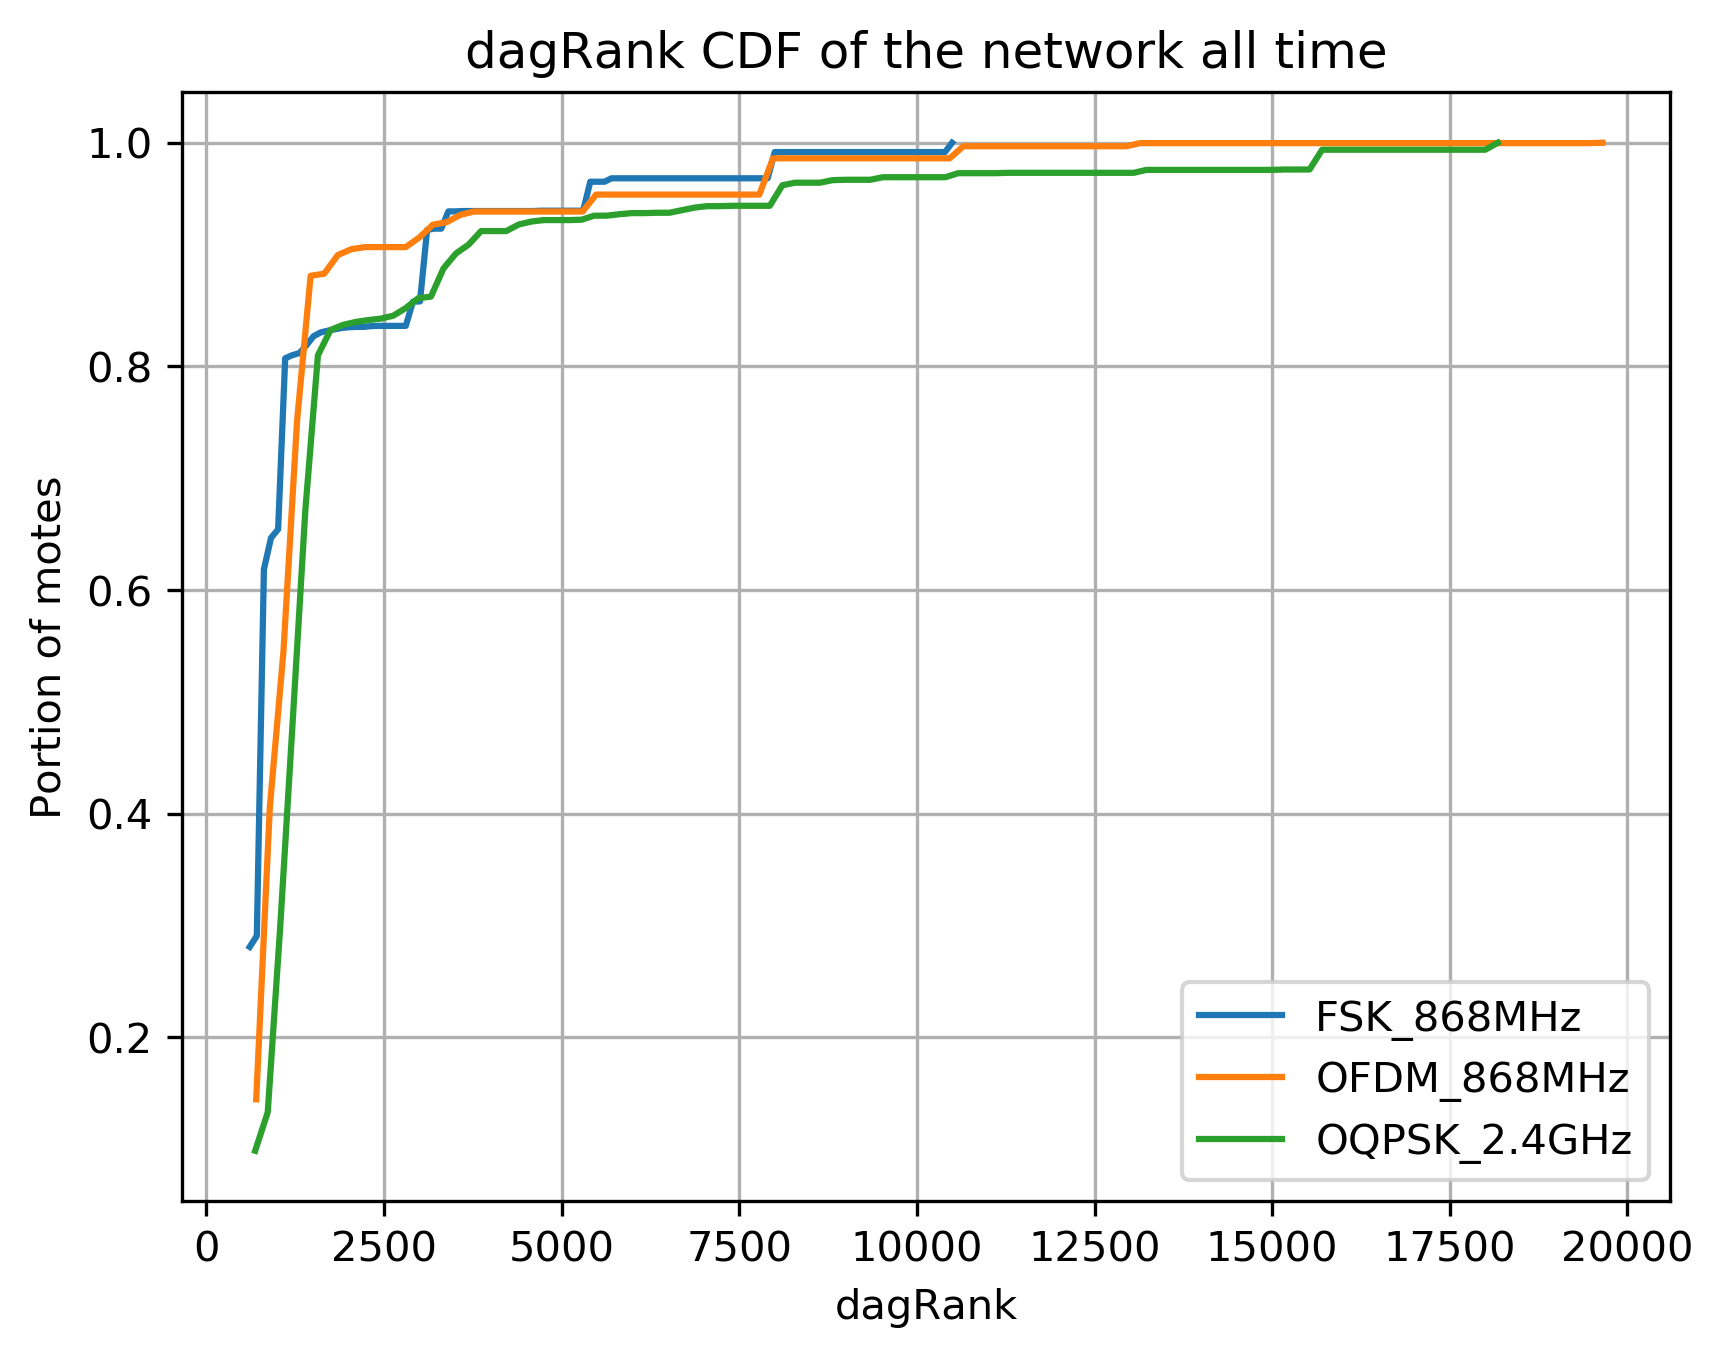
\includegraphics[width=0.90\columnwidth]{dagRank_cdf_plot_full}
	\caption{CDF of DAG Rank in the network} 
    \label{fig:{dagRank_cdf_plot_full}}
\end{figure}




\mina{mention the exact tx power levels you are using}
\begin{table*}[t]
 \caption {Battery Life - assuming 2 AA batteries with total 3V and 4.2 wh capacity} \label{tab:energy_table} 
 \begin{center}
\begin{tabular}{lllllllll}
      & Total DC & Tx DC (measured) &  \begin{tabular}[c]{@{}l@{}}RX DC\\ (estimated)\end{tabular} & \begin{tabular}[c]{@{}l@{}}Tx Current \\ (mA)\end{tabular} & \begin{tabular}[c]{@{}l@{}}Rx Current\\  (mA)\end{tabular} & \begin{tabular}[c]{@{}l@{}}Tx Power Consuption \\ (wh)\end{tabular} & \begin{tabular}[c]{@{}l@{}}Rx Power Consumption\\  (wh)\end{tabular} & \begin{tabular}[c]{@{}l@{}}Battery lifetime\\  (days)\end{tabular} \\
\fsk   & 0,02     & 0,00225          & 0,01775                                                     & 62                                                         & 28                                                         & 0,186                                                               & 0,084                                                                & 251,4997                                                           \\
\ofdm  & 0,00875  & 0,000375         & 0,008375                                                    & 62                                                         & 28                                                         & 0,186                                                               & 0,084                                                                & 872,3785                                                           \\
\oqpsk & 0,0077   & 0,0005           & 0,0072                                                      & 24                                                         & 20                                                         & 0,072                                                               & 0,06                                                                 & 2607,892                                                          
\end{tabular}
\end{center}
\end{table*}
%------------------------------------------------------------------------------
\section{Discussion}
\label{sec:discussion}
\begin{table*}[t]
 \caption {6TiSCH performance ranking for each setting} \label{tab:summary}
\begin{tabular}{lllllllll}
      & network fomration speed. & energy & latency & buffer effeciency & pdr &  &  &  \\
\fsk   & 1                        & 3      & 1       & 1                 & 1   &  &  &  \\
\ofdm  & 1                        & 2      & 2       & 1                 & 2   &  &  &  \\
\oqpsk & 3                        & 1      & 3       & 2                 & 1   &  &  & 
\end{tabular}
\end{table*}


%\begin{figure}
%	\centering
%	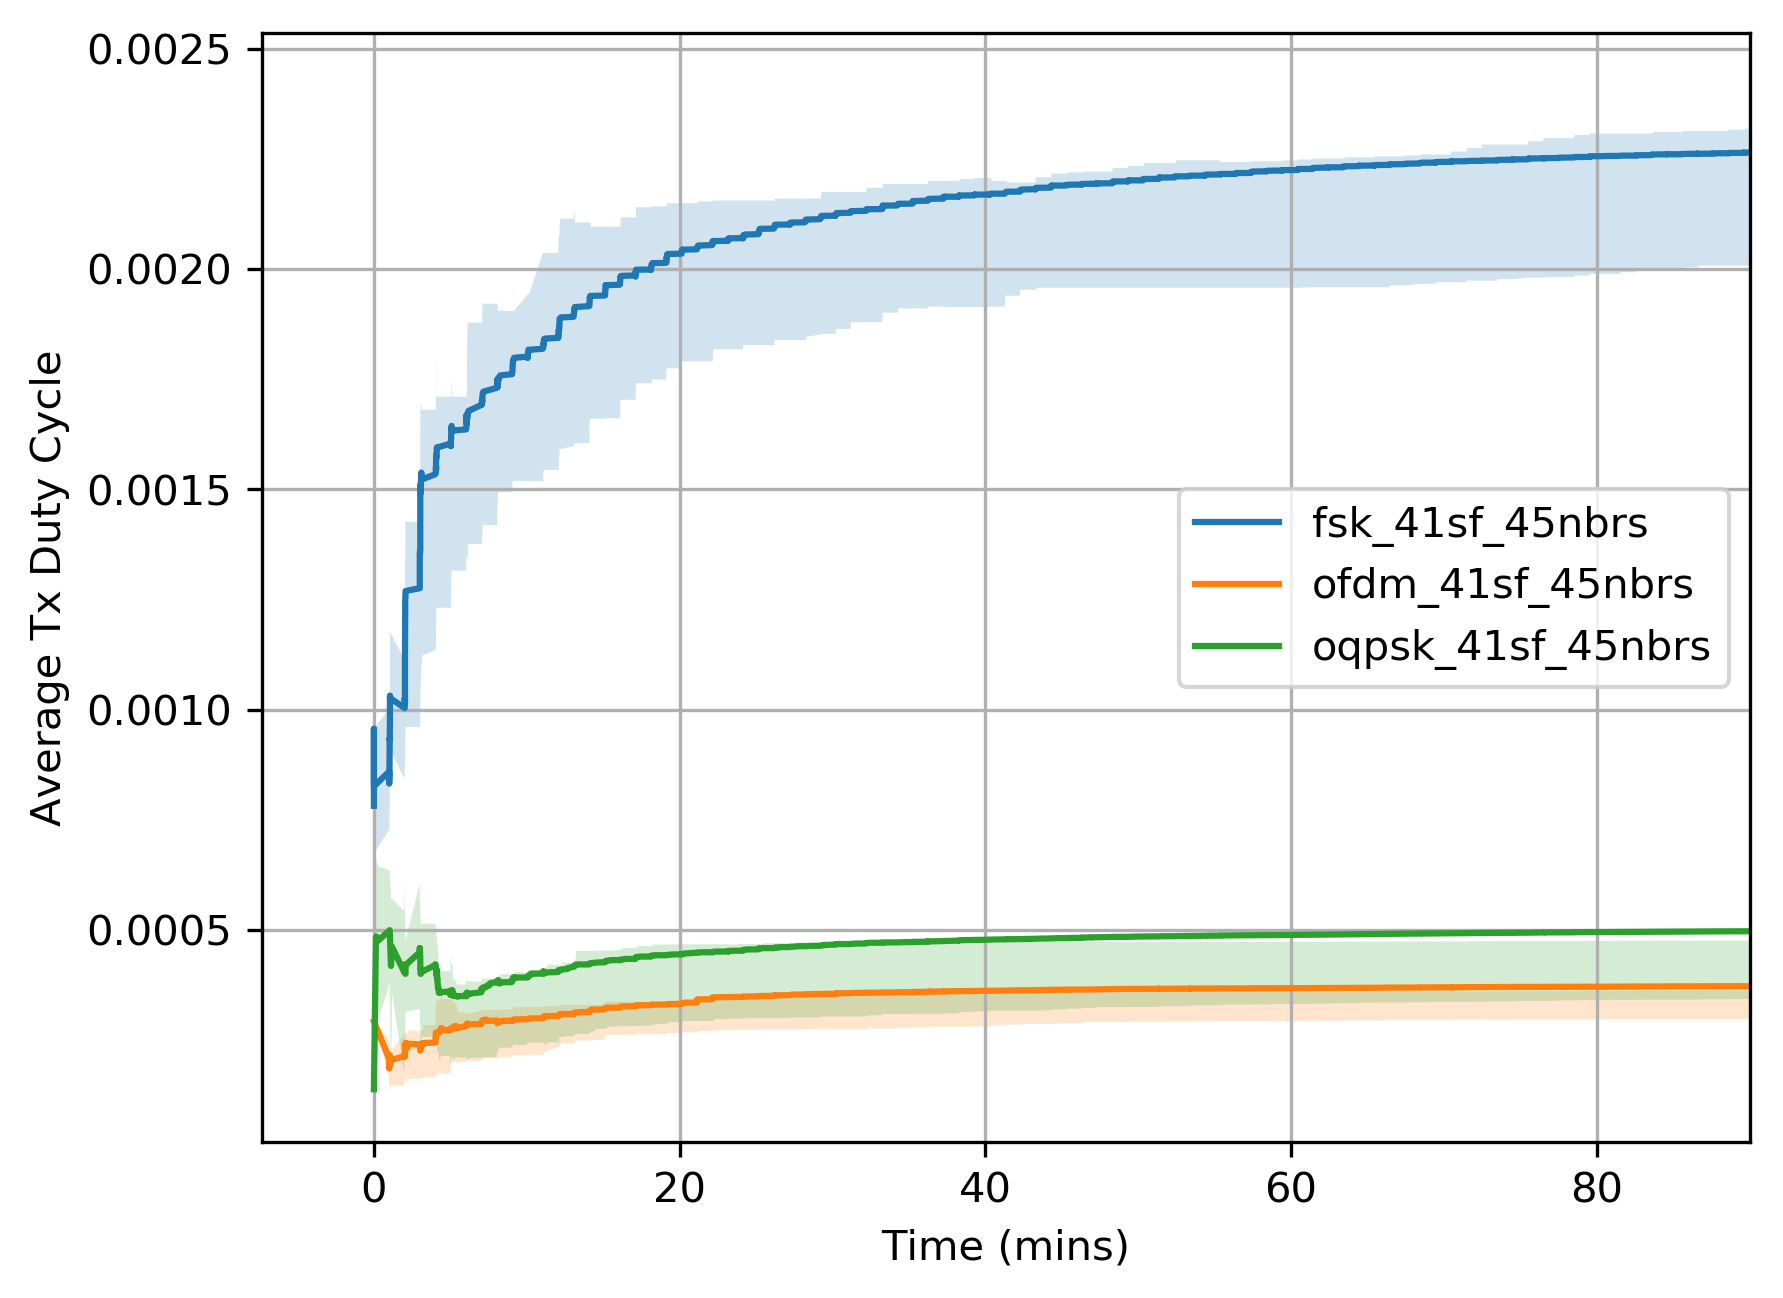
\includegraphics[width=0.90\columnwidth]{avg_avg_dutyCycleTx_plot}
%	\caption{Average transmission duty cycle}
%   \label{fig:avg_avg_dutyCycleTx_plot}
%\end{figure}

%------------------------------------------------------------------------------

\printbibliography

%==============================================================================
\end{document}

%==============================================================================
\section{Summary}

The experiments evaluate the impact of utilization of different radio access technologies at the physical layer of the 6TiSCH stack.
\begin{itemize}
    \item FSK 1 in the subghz band
    \item OFDM 1 MCS3 in the subghz band
    \item OQPSK in the 2.4 GHz band
\end{itemize}

The stack performance is evaluated at a end-to-end looking at  KPIs relevant to an SLA for a critical infrastructure, namely:
\begin{itemize}
    \item Network formation time: defined as CDF of time to first packet from all connected motes within a 30 minute time span.
    \item Reliability: defined in terms of PDR
    \item Quality of Service: defined as traffic latency
    \item Battery lifetime: expected lifetime with a power supply of 2 AA batteries.
    \item Resilience: defined as combination of two metrics: PDR of connected motes and ratio of disconnected motes (i.e. motes that were once connected) after sudden total failure of 10\% of the motes in the network (fixed set). 
\end{itemize}
    
Furthermore, the stack performance on top of each radio is evaluated at system-level for the following scenarios:
\begin{itemize}
    \item Increased traffic demand (by 300\%)
    \item Lower Network size and density (by 50\%)
\end{itemize}

%==============================================================================
\section{Draft outline}

\begin{enumerate}
    \item We explore the performance of the 6TiSCH stack in heterogeneous radio settings and we comment on the following aspects of the stack performance: network formation, reliability, quality of service, and power consumption. We observe the following. \item FSK leads to faster network formation (section \ref{sec:network_formation}). 
    \item However, FSK , as robust as it is, can lead to overall lower end-to-end reliability , which is contrary to the case of OFDM (section \ref{sec:reliability}) 
    \item Despite the lower PDR of the 6TiSCH stack in top of FSK, it shows much more end-to-end stable latency. (section \ref{sec:quality_of_service})
    \item Shorter range radios , even though they consume less energy in principle, they have a side effect as they can lead to the occupancy of the packet memory buffer due to consistent re-transmissions. This could risk reaching buffer overflow as network traffic increases. (section \ref{sec:quality_of_service})
    \item Furthermore, higher reliability of OFDM does not mean higher resilience. 
    Even though OFDM shows 99.6-100\% PDR on average compared to 99.0-99.5\% average PDR for FSK, FSK shows the best resilience in terms of PDR maintenance.  
    FSK result into a higher network degree which risks reaching limits of allocated memory buffers allocated for storage of neighbor information (section \ref{sec:resilience})
    \item Despite the advantages of FSK for end-to-end latency and network formation speed, its power consumption present a significant drawback. Also, despite the higher bitrate of OFDM compared to OQPSK, it ends up consuming similar duty cycles (b/c of re-transmissions?) (section \ref{sec:battery_lifetime})
\end{enumerate}

\begin{figure}
	\centering
	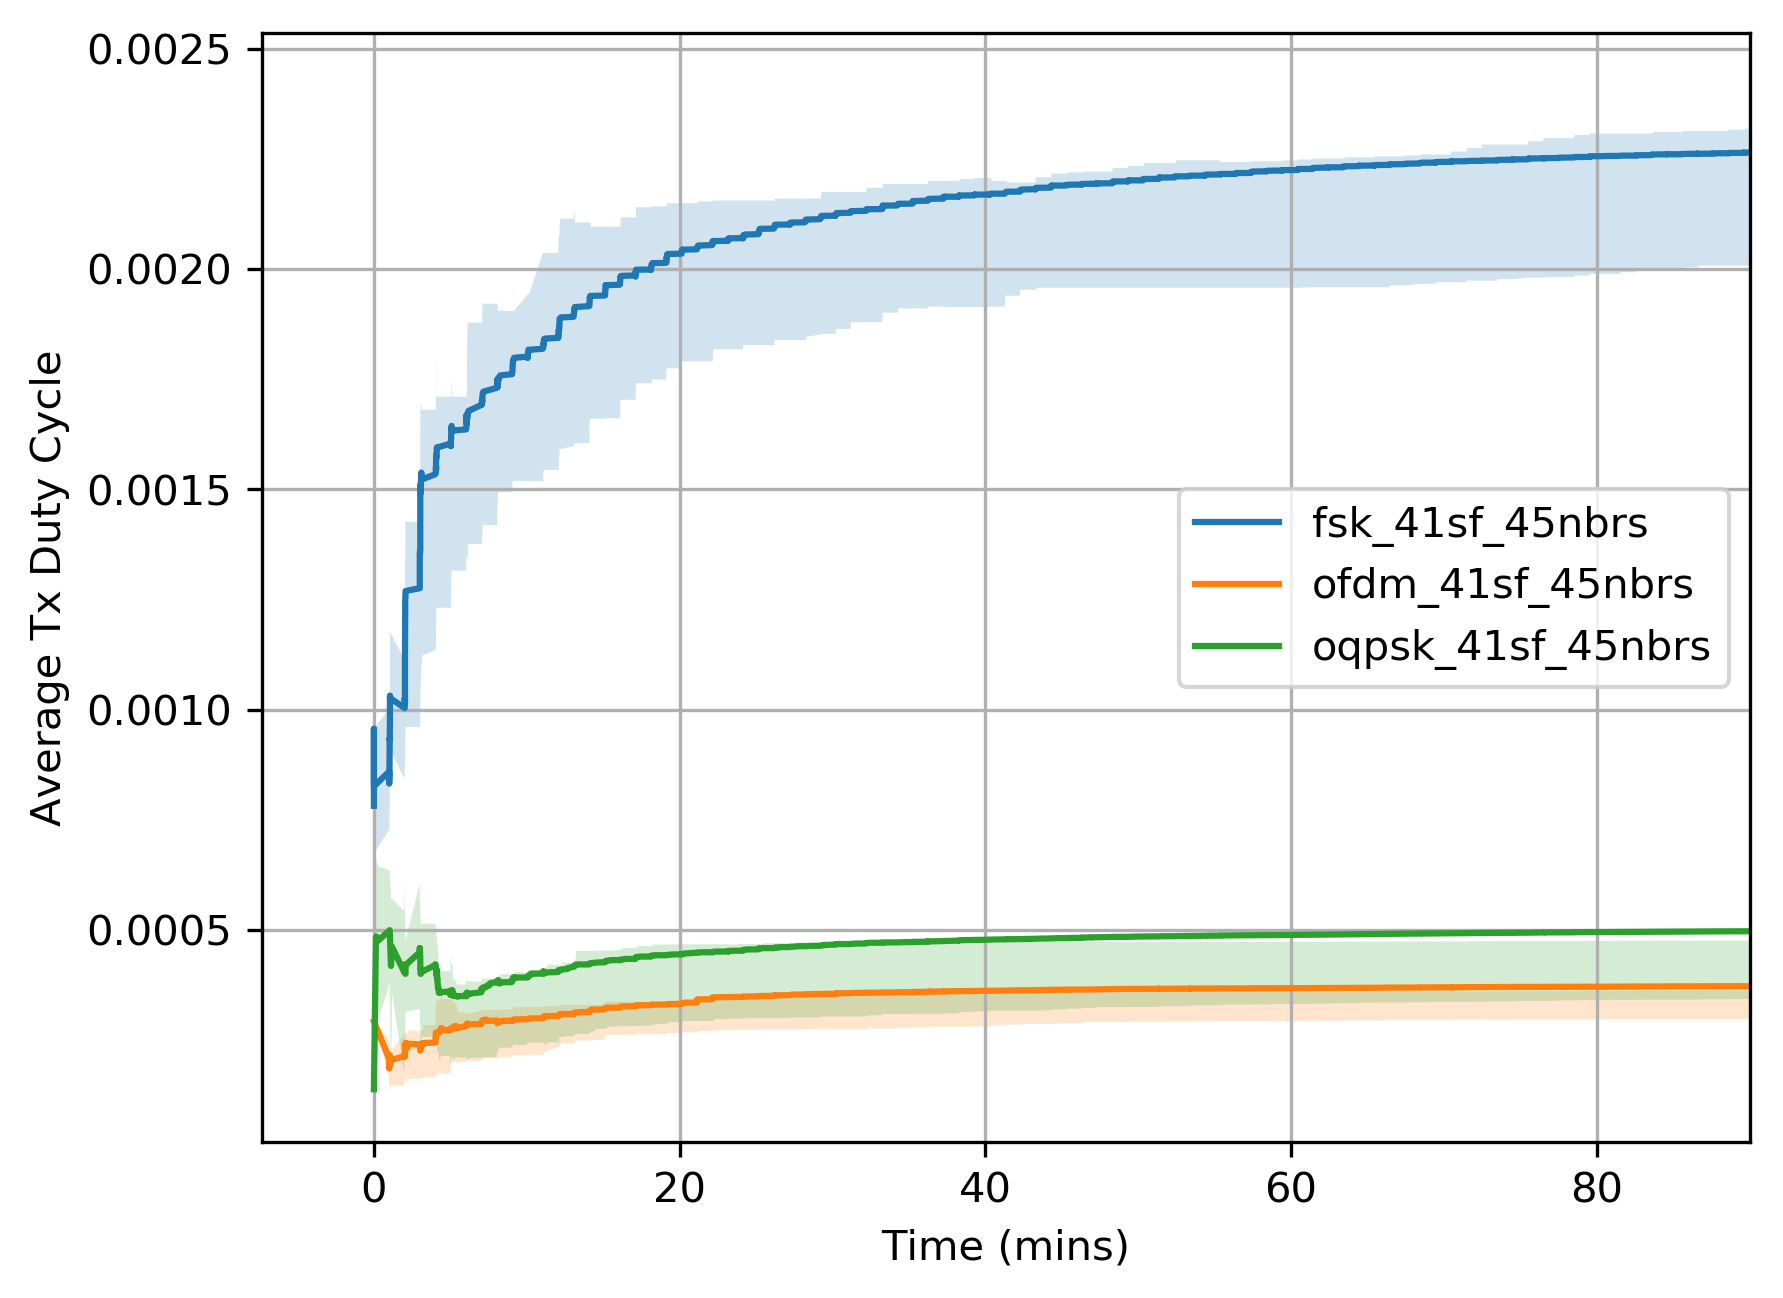
\includegraphics[width=0.90\columnwidth]{avg_avg_dutyCycleTx_plot}
	\caption{Average duty cycle. Shaded curves represent the majority of the distribution (interquartile range).}
    \label{fig:avg_avg_dutyCycleTx_plot}
\end{figure}